
\begin{frame}[noframenumbering]{comparaison avec SIFT opencv}
  \label{sift-appendix}
  \note{sift est vraiment nulle comparé à notre algo}
\begin{center}
    \begin{minipage}{0.48\textwidth}
        \onslide<1->{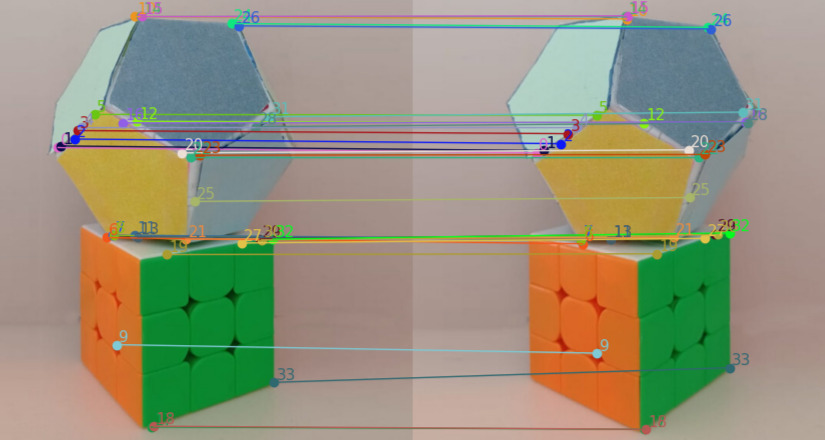
\includegraphics[width=\linewidth]{capture/app_complet_2.jpeg}\\
        \centering\scriptsize Algorithme personnalisé}
    \end{minipage}
    \hfill
    \begin{minipage}{0.48\textwidth}
        \onslide<2->{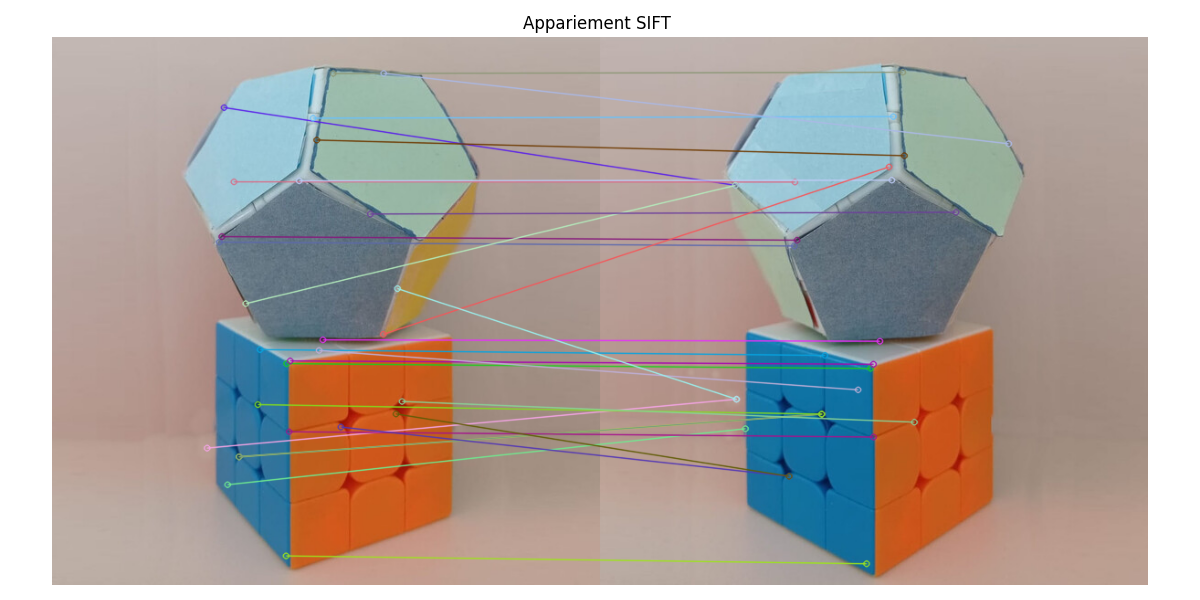
\includegraphics[width=\linewidth]{capture/sift.png}\\
        \centering\scriptsize SIFT}
    \end{minipage}
    \end{center}
\end{frame}

\begin{frame}[noframenumbering]{Exemple Moravec}
  \label{moravec-appendix}
  \centering
  \begin{tikzpicture}
    \node[anchor=south west,inner sep=0] (image) at (0,0) {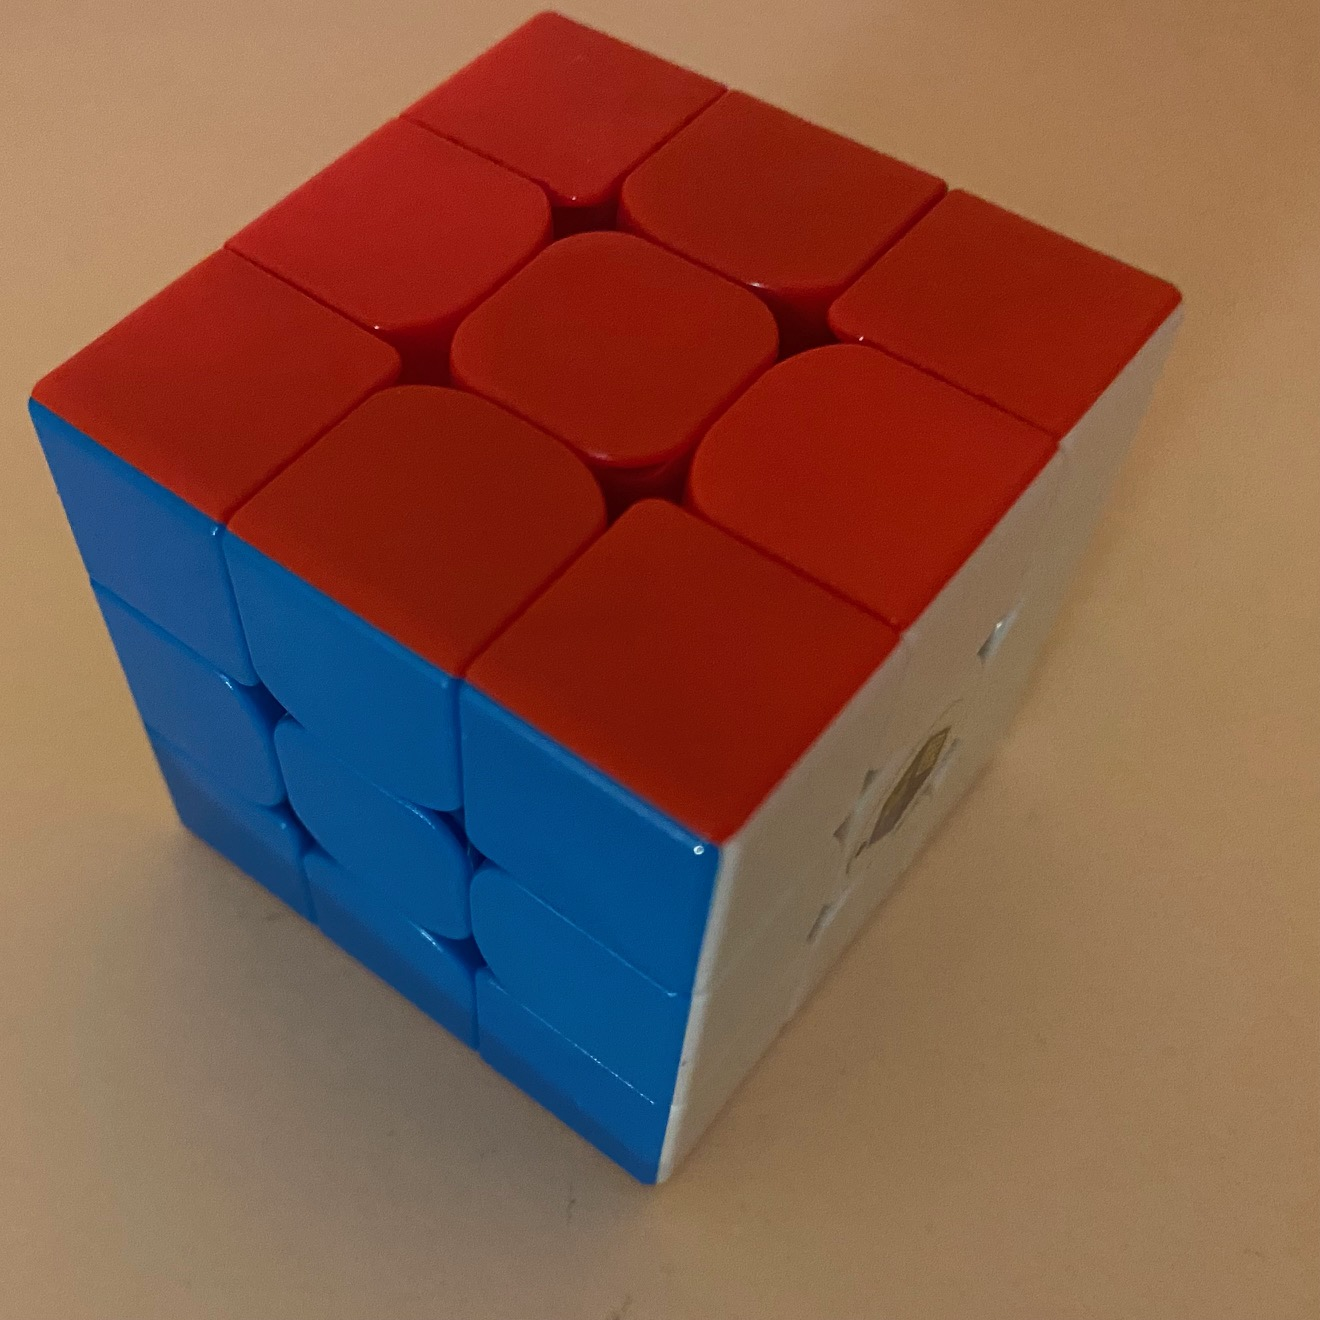
\includegraphics[width=0.5\textwidth]{capture/rub_rouge.jpg}};
    \only<2>{\draw[red, thick] (1,4.5) rectangle (2,5.5);}     % rectangle cible
  \end{tikzpicture}
\end{frame}

\begin{frame}[noframenumbering]
  \note{
    Voici une animation de l’évolution de la détection avec l’algorithme de Moravec.

    On visualise étape par étape comment les coins apparaissent au fur et à mesure.

    Ce genre de visualisation aide à comprendre la sensibilité de l’algorithme selon l’image et les paramètres.
  }
  \centering
  \begin{overlayarea}{0.9\linewidth}{4cm}
    \vspace*{-1cm}
    \hspace*{-1cm}
    \begin{tikzpicture}[x=0.75pt,y=0.75pt,yscale=-1,xscale=1, scale=2]
      \only<1>{
%Shape: Rectangle [id:dp855744465122586] 
\draw  [color={rgb, 255:red, 0; green, 0; blue, 0 }  ,draw opacity=1 ][fill={rgb, 255:red, 200; green, 43; blue, 43 }  ,fill opacity=0.23 ] (279.6,109) -- (299.6,109) -- (299.6,129) -- (279.6,129) -- cycle ;
%Shape: Rectangle [id:dp8201664290630494] 
\draw  [color={rgb, 255:red, 0; green, 0; blue, 0 }  ,draw opacity=1 ][fill={rgb, 255:red, 200; green, 43; blue, 43 }  ,fill opacity=0.64 ] (299.6,129) -- (319.6,129) -- (319.6,149) -- (299.6,149) -- cycle ;
%Shape: Rectangle [id:dp8273756646818722] 
\draw  [color={rgb, 255:red, 0; green, 0; blue, 0 }  ,draw opacity=1 ][fill={rgb, 255:red, 200; green, 43; blue, 43 }  ,fill opacity=0.64 ] (279.6,129) -- (299.6,129) -- (299.6,149) -- (279.6,149) -- cycle ;
%Shape: Rectangle [id:dp6720526871451368] 
\draw  [color={rgb, 255:red, 0; green, 0; blue, 0 }  ,draw opacity=1 ][fill={rgb, 255:red, 200; green, 43; blue, 43 }  ,fill opacity=0.69 ] (299.6,149) -- (319.6,149) -- (319.6,169) -- (299.6,169) -- cycle ;
%Shape: Rectangle [id:dp21990750654974778] 
\draw  [color={rgb, 255:red, 0; green, 0; blue, 0 }  ,draw opacity=1 ][fill={rgb, 255:red, 200; green, 43; blue, 43 }  ,fill opacity=0.68 ] (319.6,129) -- (339.6,129) -- (339.6,149) -- (319.6,149) -- cycle ;
%Shape: Rectangle [id:dp07109720325756996] 
\draw  [color={rgb, 255:red, 0; green, 0; blue, 0 }  ,draw opacity=1 ][fill={rgb, 255:red, 200; green, 43; blue, 43 }  ,fill opacity=0.32 ] (299.6,89) -- (319.6,89) -- (319.6,109) -- (299.6,109) -- cycle ;
%Shape: Rectangle [id:dp9795028573738183] 
\draw  [color={rgb, 255:red, 0; green, 0; blue, 0 }  ,draw opacity=1 ][fill={rgb, 255:red, 200; green, 43; blue, 43 }  ,fill opacity=0.64 ] (299.6,109) -- (319.6,109) -- (319.6,129) -- (299.6,129) -- cycle ;
%Shape: Rectangle [id:dp5174606270935156] 
\draw  [color={rgb, 255:red, 0; green, 0; blue, 0 }  ,draw opacity=1 ][fill={rgb, 255:red, 200; green, 43; blue, 43 }  ,fill opacity=0.23 ] (239.6,69) -- (259.6,69) -- (259.6,89) -- (239.6,89) -- cycle ;
%Shape: Rectangle [id:dp003251435331488195] 
\draw  [color={rgb, 255:red, 0; green, 0; blue, 0 }  ,draw opacity=1 ][fill={rgb, 255:red, 200; green, 43; blue, 43 }  ,fill opacity=0.21 ] (259.6,89) -- (279.6,89) -- (279.6,109) -- (259.6,109) -- cycle ;
%Shape: Rectangle [id:dp12978711061445025] 
\draw  [color={rgb, 255:red, 0; green, 0; blue, 0 }  ,draw opacity=1 ][fill={rgb, 255:red, 200; green, 43; blue, 43 }  ,fill opacity=0.25 ] (239.6,89) -- (259.6,89) -- (259.6,109) -- (239.6,109) -- cycle ;
%Shape: Rectangle [id:dp11386610015932308] 
\draw  [color={rgb, 255:red, 0; green, 0; blue, 0 }  ,draw opacity=1 ][fill={rgb, 255:red, 200; green, 43; blue, 43 }  ,fill opacity=0.28 ] (239.6,109) -- (259.6,109) -- (259.6,129) -- (239.6,129) -- cycle ;
%Shape: Rectangle [id:dp31730737510449536] 
\draw  [color={rgb, 255:red, 0; green, 0; blue, 0 }  ,draw opacity=1 ][fill={rgb, 255:red, 200; green, 43; blue, 43 }  ,fill opacity=0.66 ] (259.6,129) -- (279.6,129) -- (279.6,149) -- (259.6,149) -- cycle ;
%Shape: Rectangle [id:dp0039535950874963754] 
\draw  [color={rgb, 255:red, 0; green, 0; blue, 0 }  ,draw opacity=1 ][fill={rgb, 255:red, 200; green, 43; blue, 43 }  ,fill opacity=0.77 ] (279.6,149) -- (299.6,149) -- (299.6,169) -- (279.6,169) -- cycle ;
%Shape: Rectangle [id:dp5148350575823291] 
\draw  [color={rgb, 255:red, 0; green, 0; blue, 0 }  ,draw opacity=1 ][fill={rgb, 255:red, 200; green, 43; blue, 43 }  ,fill opacity=0.24 ] (259.6,109) -- (279.6,109) -- (279.6,129) -- (259.6,129) -- cycle ;
%Shape: Rectangle [id:dp36043744827539115] 
\draw  [color={rgb, 255:red, 0; green, 0; blue, 0 }  ,draw opacity=1 ][fill={rgb, 255:red, 200; green, 43; blue, 43 }  ,fill opacity=0.26 ] (259.6,69) -- (279.6,69) -- (279.6,89) -- (259.6,89) -- cycle ;
%Shape: Rectangle [id:dp3332412201524424] 
\draw  [color={rgb, 255:red, 0; green, 0; blue, 0 }  ,draw opacity=1 ][fill={rgb, 255:red, 200; green, 43; blue, 43 }  ,fill opacity=0.22 ] (279.6,89) -- (299.6,89) -- (299.6,109) -- (279.6,109) -- cycle ;
%Shape: Rectangle [id:dp49757845918426946] 
\draw  [color={rgb, 255:red, 0; green, 0; blue, 0 }  ,draw opacity=1 ][fill={rgb, 255:red, 200; green, 43; blue, 43 }  ,fill opacity=0.29 ] (279.6,69) -- (299.6,69) -- (299.6,89) -- (279.6,89) -- cycle ;
%Shape: Rectangle [id:dp1948054383738922] 
\draw  [color={rgb, 255:red, 0; green, 0; blue, 0 }  ,draw opacity=1 ][fill={rgb, 255:red, 200; green, 43; blue, 43 }  ,fill opacity=0.28 ] (299.6,69) -- (319.6,69) -- (319.6,89) -- (299.6,89) -- cycle ;
%Shape: Rectangle [id:dp5908482157161481] 
\draw  [color={rgb, 255:red, 0; green, 0; blue, 0 }  ,draw opacity=1 ][fill={rgb, 255:red, 200; green, 43; blue, 43 }  ,fill opacity=0.65 ] (319.6,109) -- (339.6,109) -- (339.6,129) -- (319.6,129) -- cycle ;
%Shape: Rectangle [id:dp8244027566618196] 
\draw  [color={rgb, 255:red, 0; green, 0; blue, 0 }  ,draw opacity=1 ][fill={rgb, 255:red, 200; green, 43; blue, 43 }  ,fill opacity=0.64 ] (239.6,129) -- (259.6,129) -- (259.6,149) -- (239.6,149) -- cycle ;
%Shape: Rectangle [id:dp29418903051156065] 
\draw  [color={rgb, 255:red, 0; green, 0; blue, 0 }  ,draw opacity=1 ][fill={rgb, 255:red, 200; green, 43; blue, 43 }  ,fill opacity=0.73 ] (239.6,149) -- (259.6,149) -- (259.6,169) -- (239.6,169) -- cycle ;
%Shape: Rectangle [id:dp03059484266780088] 
\draw  [color={rgb, 255:red, 0; green, 0; blue, 0 }  ,draw opacity=1 ][fill={rgb, 255:red, 200; green, 43; blue, 43 }  ,fill opacity=0.74 ] (259.6,149) -- (279.6,149) -- (279.6,169) -- (259.6,169) -- cycle ;
%Shape: Rectangle [id:dp15824841679231605] 
\draw  [color={rgb, 255:red, 0; green, 0; blue, 0 }  ,draw opacity=1 ][fill={rgb, 255:red, 200; green, 43; blue, 43 }  ,fill opacity=0.68 ] (319.6,149) -- (339.6,149) -- (339.6,169) -- (319.6,169) -- cycle ;
%Shape: Rectangle [id:dp5219374564422655] 
\draw  [color={rgb, 255:red, 0; green, 0; blue, 0 }  ,draw opacity=1 ][fill={rgb, 255:red, 200; green, 43; blue, 43 }  ,fill opacity=0.7 ] (319.6,69) -- (339.6,69) -- (339.6,89) -- (319.6,89) -- cycle ;
%Shape: Rectangle [id:dp41832573855226485] 
\draw  [color={rgb, 255:red, 0; green, 0; blue, 0 }  ,draw opacity=1 ][fill={rgb, 255:red, 200; green, 43; blue, 43 }  ,fill opacity=0.63 ] (319.6,89) -- (339.6,89) -- (339.6,109) -- (319.6,109) -- cycle ;
%Shape: Rectangle [id:dp4512036699306804] 
\draw  [color={rgb, 255:red, 255; green, 255; blue, 255 }  ,draw opacity=1 ] (209,54.5) -- (451,54.5) -- (451,190.5) -- (209,190.5) -- cycle ;
%Shape: Rectangle [id:dp30277857918883444] 
\draw  [color={rgb, 255:red, 222; green, 195; blue, 14 }  ,draw opacity=1 ][fill={rgb, 255:red, 192; green, 177; blue, 255 }  ,fill opacity=0.34 ] (259.6,335) -- (279.6,335) -- (279.6,355) -- (259.6,355) -- cycle ;

% Text Node
\draw (304.8,136) node [anchor=north west][inner sep=0.75pt]  [font=\footnotesize] [align=left] {64};
% Text Node
\draw (324.8,155.2) node [anchor=north west][inner sep=0.75pt]  [font=\footnotesize] [align=left] {69};
% Text Node
\draw (305.2,115.6) node [anchor=north west][inner sep=0.75pt]  [font=\footnotesize] [align=left] {65};
% Text Node
\draw (305.2,95.6) node [anchor=north west][inner sep=0.75pt]  [font=\footnotesize] [align=left] {32};
% Text Node
\draw (285.2,95.6) node [anchor=north west][inner sep=0.75pt]  [font=\footnotesize] [align=left] {22};
% Text Node
\draw (325.2,115.6) node [anchor=north west][inner sep=0.75pt]  [font=\footnotesize] [align=left] {65};
% Text Node
\draw (244.4,76) node [anchor=north west][inner sep=0.75pt]  [font=\footnotesize] [align=left] {23};
% Text Node
\draw (265.2,96) node [anchor=north west][inner sep=0.75pt]  [font=\footnotesize] [align=left] {21};
% Text Node
\draw (244.8,95.6) node [anchor=north west][inner sep=0.75pt]  [font=\footnotesize] [align=left] {25};
% Text Node
\draw (264.8,116.4) node [anchor=north west][inner sep=0.75pt]  [font=\footnotesize] [align=left] {24};
% Text Node
\draw (284.8,135.6) node [anchor=north west][inner sep=0.75pt]  [font=\footnotesize] [align=left] {64};
% Text Node
\draw (304.8,155.2) node [anchor=north west][inner sep=0.75pt]  [font=\footnotesize] [align=left] {69};
% Text Node
\draw (264.4,75.6) node [anchor=north west][inner sep=0.75pt]  [font=\footnotesize] [align=left] {26};
% Text Node
\draw (285.2,75.6) node [anchor=north west][inner sep=0.75pt]  [font=\footnotesize] [align=left] {29};
% Text Node
\draw (304.8,75.2) node [anchor=north west][inner sep=0.75pt]  [font=\footnotesize] [align=left] {28};
% Text Node
\draw (324.8,95.2) node [anchor=north west][inner sep=0.75pt]  [font=\footnotesize] [align=left] {63};
% Text Node
\draw (324.8,76.8) node [anchor=north west][inner sep=0.75pt]  [font=\footnotesize] [align=left] {70};
% Text Node
\draw (244.8,115.6) node [anchor=north west][inner sep=0.75pt]  [font=\footnotesize] [align=left] {28};
% Text Node
\draw (264.8,135.6) node [anchor=north west][inner sep=0.75pt]  [font=\footnotesize] [align=left] {66};
% Text Node
\draw (284.8,155.2) node [anchor=north west][inner sep=0.75pt]  [font=\footnotesize] [align=left] {77};
% Text Node
\draw (244,136) node [anchor=north west][inner sep=0.75pt]  [font=\footnotesize] [align=left] {63};
% Text Node
\draw (264,155.2) node [anchor=north west][inner sep=0.75pt]  [font=\footnotesize] [align=left] {74};
% Text Node
\draw (245.2,155.6) node [anchor=north west][inner sep=0.75pt]  [font=\footnotesize] [align=left] {73};
% Text Node
\draw (324.8,136.4) node [anchor=north west][inner sep=0.75pt]  [font=\footnotesize] [align=left] {68};
% Text Node
\draw (285.2,116.4) node [anchor=north west][inner sep=0.75pt]  [font=\footnotesize] [align=left] {23};

\draw (355,80) node [anchor=north west][inner sep=0.75pt]  [font=\footnotesize]  {$w=2$};}
      \only<2>{
%Shape: Rectangle [id:dp34895762482355186] 
\draw  [color={rgb, 255:red, 0; green, 0; blue, 0 }  ,draw opacity=1 ][fill={rgb, 255:red, 200; green, 43; blue, 43 }  ,fill opacity=0.23 ] (279.6,109) -- (299.6,109) -- (299.6,129) -- (279.6,129) -- cycle ;
%Shape: Rectangle [id:dp3706129514955345] 
\draw  [color={rgb, 255:red, 0; green, 0; blue, 0 }  ,draw opacity=1 ][fill={rgb, 255:red, 200; green, 43; blue, 43 }  ,fill opacity=0.64 ] (299.6,129) -- (319.6,129) -- (319.6,149) -- (299.6,149) -- cycle ;
%Shape: Rectangle [id:dp7937037744108977] 
\draw  [color={rgb, 255:red, 0; green, 0; blue, 0 }  ,draw opacity=1 ][fill={rgb, 255:red, 200; green, 43; blue, 43 }  ,fill opacity=0.64 ] (279.6,129) -- (299.6,129) -- (299.6,149) -- (279.6,149) -- cycle ;
%Shape: Rectangle [id:dp20259457131157055] 
\draw  [color={rgb, 255:red, 0; green, 0; blue, 0 }  ,draw opacity=1 ][fill={rgb, 255:red, 200; green, 43; blue, 43 }  ,fill opacity=0.69 ] (299.6,149) -- (319.6,149) -- (319.6,169) -- (299.6,169) -- cycle ;
%Shape: Rectangle [id:dp4433057251733791] 
\draw  [color={rgb, 255:red, 0; green, 0; blue, 0 }  ,draw opacity=1 ][fill={rgb, 255:red, 200; green, 43; blue, 43 }  ,fill opacity=0.68 ] (319.6,129) -- (339.6,129) -- (339.6,149) -- (319.6,149) -- cycle ;
%Shape: Rectangle [id:dp6669398936433204] 
\draw  [color={rgb, 255:red, 0; green, 0; blue, 0 }  ,draw opacity=1 ][fill={rgb, 255:red, 200; green, 43; blue, 43 }  ,fill opacity=0.32 ] (299.6,89) -- (319.6,89) -- (319.6,109) -- (299.6,109) -- cycle ;
%Shape: Rectangle [id:dp21171515185264544] 
\draw  [color={rgb, 255:red, 0; green, 0; blue, 0 }  ,draw opacity=1 ][fill={rgb, 255:red, 200; green, 43; blue, 43 }  ,fill opacity=0.64 ] (299.6,109) -- (319.6,109) -- (319.6,129) -- (299.6,129) -- cycle ;
%Shape: Rectangle [id:dp06872955891721255] 
\draw  [color={rgb, 255:red, 0; green, 0; blue, 0 }  ,draw opacity=1 ][fill={rgb, 255:red, 200; green, 43; blue, 43 }  ,fill opacity=0.23 ] (239.6,69) -- (259.6,69) -- (259.6,89) -- (239.6,89) -- cycle ;
%Shape: Rectangle [id:dp31874857825881] 
\draw  [color={rgb, 255:red, 0; green, 0; blue, 0 }  ,draw opacity=1 ][fill={rgb, 255:red, 200; green, 43; blue, 43 }  ,fill opacity=0.21 ] (259.6,89) -- (279.6,89) -- (279.6,109) -- (259.6,109) -- cycle ;
%Shape: Rectangle [id:dp6824558327787323] 
\draw  [color={rgb, 255:red, 0; green, 0; blue, 0 }  ,draw opacity=1 ][fill={rgb, 255:red, 200; green, 43; blue, 43 }  ,fill opacity=0.25 ] (239.6,89) -- (259.6,89) -- (259.6,109) -- (239.6,109) -- cycle ;
%Shape: Rectangle [id:dp7485420074379594] 
\draw  [color={rgb, 255:red, 0; green, 0; blue, 0 }  ,draw opacity=1 ][fill={rgb, 255:red, 200; green, 43; blue, 43 }  ,fill opacity=0.28 ] (239.6,109) -- (259.6,109) -- (259.6,129) -- (239.6,129) -- cycle ;
%Shape: Rectangle [id:dp518076998549063] 
\draw  [color={rgb, 255:red, 0; green, 0; blue, 0 }  ,draw opacity=1 ][fill={rgb, 255:red, 200; green, 43; blue, 43 }  ,fill opacity=0.66 ] (259.6,129) -- (279.6,129) -- (279.6,149) -- (259.6,149) -- cycle ;
%Shape: Rectangle [id:dp30451200783199606] 
\draw  [color={rgb, 255:red, 0; green, 0; blue, 0 }  ,draw opacity=1 ][fill={rgb, 255:red, 200; green, 43; blue, 43 }  ,fill opacity=0.77 ] (279.6,149) -- (299.6,149) -- (299.6,169) -- (279.6,169) -- cycle ;
%Shape: Rectangle [id:dp1908549710583085] 
\draw  [color={rgb, 255:red, 0; green, 0; blue, 0 }  ,draw opacity=1 ][fill={rgb, 255:red, 200; green, 43; blue, 43 }  ,fill opacity=0.24 ] (259.6,109) -- (279.6,109) -- (279.6,129) -- (259.6,129) -- cycle ;
%Shape: Rectangle [id:dp4988144165606093] 
\draw  [color={rgb, 255:red, 0; green, 0; blue, 0 }  ,draw opacity=1 ][fill={rgb, 255:red, 200; green, 43; blue, 43 }  ,fill opacity=0.26 ] (259.6,69) -- (279.6,69) -- (279.6,89) -- (259.6,89) -- cycle ;
%Shape: Rectangle [id:dp7655450055950659] 
\draw  [color={rgb, 255:red, 0; green, 0; blue, 0 }  ,draw opacity=1 ][fill={rgb, 255:red, 200; green, 43; blue, 43 }  ,fill opacity=0.22 ] (279.6,89) -- (299.6,89) -- (299.6,109) -- (279.6,109) -- cycle ;
%Shape: Rectangle [id:dp13960350908642583] 
\draw  [color={rgb, 255:red, 0; green, 0; blue, 0 }  ,draw opacity=1 ][fill={rgb, 255:red, 200; green, 43; blue, 43 }  ,fill opacity=0.29 ] (279.6,69) -- (299.6,69) -- (299.6,89) -- (279.6,89) -- cycle ;
%Shape: Rectangle [id:dp4182608599365719] 
\draw  [color={rgb, 255:red, 0; green, 0; blue, 0 }  ,draw opacity=1 ][fill={rgb, 255:red, 200; green, 43; blue, 43 }  ,fill opacity=0.28 ] (299.6,69) -- (319.6,69) -- (319.6,89) -- (299.6,89) -- cycle ;
%Shape: Rectangle [id:dp3569567884999012] 
\draw  [color={rgb, 255:red, 0; green, 0; blue, 0 }  ,draw opacity=1 ][fill={rgb, 255:red, 200; green, 43; blue, 43 }  ,fill opacity=0.65 ] (319.6,109) -- (339.6,109) -- (339.6,129) -- (319.6,129) -- cycle ;
%Shape: Rectangle [id:dp28676610010827] 
\draw  [color={rgb, 255:red, 0; green, 0; blue, 0 }  ,draw opacity=1 ][fill={rgb, 255:red, 200; green, 43; blue, 43 }  ,fill opacity=0.64 ] (239.6,129) -- (259.6,129) -- (259.6,149) -- (239.6,149) -- cycle ;
%Shape: Rectangle [id:dp45600868944371487] 
\draw  [color={rgb, 255:red, 0; green, 0; blue, 0 }  ,draw opacity=1 ][fill={rgb, 255:red, 200; green, 43; blue, 43 }  ,fill opacity=0.73 ] (239.6,149) -- (259.6,149) -- (259.6,169) -- (239.6,169) -- cycle ;
%Shape: Rectangle [id:dp8145428819349263] 
\draw  [color={rgb, 255:red, 0; green, 0; blue, 0 }  ,draw opacity=1 ][fill={rgb, 255:red, 200; green, 43; blue, 43 }  ,fill opacity=0.74 ] (259.6,149) -- (279.6,149) -- (279.6,169) -- (259.6,169) -- cycle ;
%Shape: Rectangle [id:dp7078836921241948] 
\draw  [color={rgb, 255:red, 0; green, 0; blue, 0 }  ,draw opacity=1 ][fill={rgb, 255:red, 200; green, 43; blue, 43 }  ,fill opacity=0.68 ] (319.6,149) -- (339.6,149) -- (339.6,169) -- (319.6,169) -- cycle ;
%Shape: Rectangle [id:dp8396418073196056] 
\draw  [color={rgb, 255:red, 0; green, 0; blue, 0 }  ,draw opacity=1 ][fill={rgb, 255:red, 200; green, 43; blue, 43 }  ,fill opacity=0.7 ] (319.6,69) -- (339.6,69) -- (339.6,89) -- (319.6,89) -- cycle ;
%Shape: Rectangle [id:dp9348793553111198] 
\draw  [color={rgb, 255:red, 0; green, 0; blue, 0 }  ,draw opacity=1 ][fill={rgb, 255:red, 200; green, 43; blue, 43 }  ,fill opacity=0.63 ] (319.6,89) -- (339.6,89) -- (339.6,109) -- (319.6,109) -- cycle ;
%Shape: Rectangle [id:dp10953260736468606] 
\draw  [color={rgb, 255:red, 30; green, 14; blue, 222 }  ,draw opacity=1 ][fill={rgb, 255:red, 192; green, 177; blue, 255 }  ,fill opacity=0.34 ] (279.6,109) -- (299.6,109) -- (299.6,129) -- (279.6,129) -- cycle ;
%Shape: Rectangle [id:dp7457156202929361] 
\draw  [color={rgb, 255:red, 255; green, 255; blue, 255 }  ,draw opacity=1 ] (209,54.5) -- (451,54.5) -- (451,190.5) -- (209,190.5) -- cycle ;
%Shape: Rectangle [id:dp4886950260713504] 
\draw  [color={rgb, 255:red, 222; green, 195; blue, 14 }  ,draw opacity=1 ][fill={rgb, 255:red, 192; green, 177; blue, 255 }  ,fill opacity=0.34 ] (239.6,109) -- (259.6,109) -- (259.6,129) -- (239.6,129) -- cycle ;
%Shape: Rectangle [id:dp7097656602066365] 
\draw  [color={rgb, 255:red, 222; green, 195; blue, 14 }  ,draw opacity=1 ][fill={rgb, 255:red, 192; green, 177; blue, 255 }  ,fill opacity=0.34 ] (259.6,335) -- (279.6,335) -- (279.6,355) -- (259.6,355) -- cycle ;


\draw (304.8,136) node [anchor=north west][inner sep=0.75pt]  [font=\footnotesize] [align=left] {64};
% Text Node
\draw (324.8,155.2) node [anchor=north west][inner sep=0.75pt]  [font=\footnotesize] [align=left] {69};
% Text Node
\draw (305.2,115.6) node [anchor=north west][inner sep=0.75pt]  [font=\footnotesize] [align=left] {65};
% Text Node
\draw (305.2,95.6) node [anchor=north west][inner sep=0.75pt]  [font=\footnotesize] [align=left] {32};
% Text Node
\draw (285.2,95.6) node [anchor=north west][inner sep=0.75pt]  [font=\footnotesize] [align=left] {22};
% Text Node
\draw (325.2,115.6) node [anchor=north west][inner sep=0.75pt]  [font=\footnotesize] [align=left] {65};
% Text Node
\draw (244.4,76) node [anchor=north west][inner sep=0.75pt]  [font=\footnotesize] [align=left] {23};
% Text Node
\draw (265.2,96) node [anchor=north west][inner sep=0.75pt]  [font=\footnotesize] [align=left] {21};
% Text Node
\draw (244.8,95.6) node [anchor=north west][inner sep=0.75pt]  [font=\footnotesize] [align=left] {25};
% Text Node
\draw (264.8,116.4) node [anchor=north west][inner sep=0.75pt]  [font=\footnotesize] [align=left] {24};
% Text Node
\draw (284.8,135.6) node [anchor=north west][inner sep=0.75pt]  [font=\footnotesize] [align=left] {64};
% Text Node
\draw (304.8,155.2) node [anchor=north west][inner sep=0.75pt]  [font=\footnotesize] [align=left] {69};
% Text Node
\draw (264.4,75.6) node [anchor=north west][inner sep=0.75pt]  [font=\footnotesize] [align=left] {26};
% Text Node
\draw (285.2,75.6) node [anchor=north west][inner sep=0.75pt]  [font=\footnotesize] [align=left] {29};
% Text Node
\draw (304.8,75.2) node [anchor=north west][inner sep=0.75pt]  [font=\footnotesize] [align=left] {28};
% Text Node
\draw (324.8,95.2) node [anchor=north west][inner sep=0.75pt]  [font=\footnotesize] [align=left] {63};
% Text Node
\draw (324.8,76.8) node [anchor=north west][inner sep=0.75pt]  [font=\footnotesize] [align=left] {70};
% Text Node
\draw (244.8,115.6) node [anchor=north west][inner sep=0.75pt]  [font=\footnotesize] [align=left] {28};
% Text Node
\draw (264.8,135.6) node [anchor=north west][inner sep=0.75pt]  [font=\footnotesize] [align=left] {66};
% Text Node
\draw (284.8,155.2) node [anchor=north west][inner sep=0.75pt]  [font=\footnotesize] [align=left] {77};
% Text Node
\draw (244,136) node [anchor=north west][inner sep=0.75pt]  [font=\footnotesize] [align=left] {63};
% Text Node
\draw (264,155.2) node [anchor=north west][inner sep=0.75pt]  [font=\footnotesize] [align=left] {74};
% Text Node
\draw (245.2,155.6) node [anchor=north west][inner sep=0.75pt]  [font=\footnotesize] [align=left] {73};
% Text Node
\draw (324.8,136.4) node [anchor=north west][inner sep=0.75pt]  [font=\footnotesize] [align=left] {68};
% Text Node
\draw (285.2,116.4) node [anchor=north west][inner sep=0.75pt]  [font=\footnotesize] [align=left] {23};
% Text Node


\draw (355,80) node [anchor=north west][inner sep=0.75pt]  [font=\footnotesize]  {$w=2$};
% Text Node
\draw (355,135.4) node [anchor=north west][inner sep=0.75pt]  [font=\footnotesize]  {$i=-2$};
% Text Node
\draw (355,108.8) node [anchor=north west][inner sep=0.75pt]  [font=\footnotesize]  {$dx=1,\ dy=0$};
% Text Node
\draw (355,125.27) node [anchor=north west][inner sep=0.75pt]  [font=\footnotesize,color={rgb, 255:red, 72; green, 36; blue, 227 }  ,opacity=1 ] [align=left] {\textcolor[rgb]{0.55,0.64,0.02}{pixel comparé}};
% Text Node
\draw (355,98.13) node [anchor=north west][inner sep=0.75pt]  [font=\footnotesize,opacity=1 ] [align=left] {direction horizontal};
% Text Node
\draw (355.3,154.4) node [anchor=north west][inner sep=0.75pt]  [font=\footnotesize]  {$S=28$};
% Text Node
\draw (383.3,154.0) node [anchor=north west][inner sep=0.75pt]  [font=\footnotesize]  {$S^{2} =784$};

% Text Node
\draw (355,117) node [anchor=north west][inner sep=0.75pt]  [font=\footnotesize,color={rgb, 255:red, 72; green, 36; blue, 227 }  ,opacity=1 ] [align=left] {pixel considéré};
% Text Node}
      \only<3>{
%Shape: Rectangle [id:dp4812352510414377] 
\draw  [color={rgb, 255:red, 0; green, 0; blue, 0 }  ,draw opacity=1 ][fill={rgb, 255:red, 200; green, 43; blue, 43 }  ,fill opacity=0.23 ] (279.6,109) -- (299.6,109) -- (299.6,129) -- (279.6,129) -- cycle ;
%Shape: Rectangle [id:dp8369925573319851] 
\draw  [color={rgb, 255:red, 0; green, 0; blue, 0 }  ,draw opacity=1 ][fill={rgb, 255:red, 200; green, 43; blue, 43 }  ,fill opacity=0.64 ] (299.6,129) -- (319.6,129) -- (319.6,149) -- (299.6,149) -- cycle ;
%Shape: Rectangle [id:dp22732928696285393] 
\draw  [color={rgb, 255:red, 0; green, 0; blue, 0 }  ,draw opacity=1 ][fill={rgb, 255:red, 200; green, 43; blue, 43 }  ,fill opacity=0.64 ] (279.6,129) -- (299.6,129) -- (299.6,149) -- (279.6,149) -- cycle ;
%Shape: Rectangle [id:dp8704034364799831] 
\draw  [color={rgb, 255:red, 0; green, 0; blue, 0 }  ,draw opacity=1 ][fill={rgb, 255:red, 200; green, 43; blue, 43 }  ,fill opacity=0.69 ] (299.6,149) -- (319.6,149) -- (319.6,169) -- (299.6,169) -- cycle ;
%Shape: Rectangle [id:dp37274322264135495] 
\draw  [color={rgb, 255:red, 0; green, 0; blue, 0 }  ,draw opacity=1 ][fill={rgb, 255:red, 200; green, 43; blue, 43 }  ,fill opacity=0.68 ] (319.6,129) -- (339.6,129) -- (339.6,149) -- (319.6,149) -- cycle ;
%Shape: Rectangle [id:dp2642638953436689] 
\draw  [color={rgb, 255:red, 0; green, 0; blue, 0 }  ,draw opacity=1 ][fill={rgb, 255:red, 200; green, 43; blue, 43 }  ,fill opacity=0.32 ] (299.6,89) -- (319.6,89) -- (319.6,109) -- (299.6,109) -- cycle ;
%Shape: Rectangle [id:dp5440385706105905] 
\draw  [color={rgb, 255:red, 0; green, 0; blue, 0 }  ,draw opacity=1 ][fill={rgb, 255:red, 200; green, 43; blue, 43 }  ,fill opacity=0.64 ] (299.6,109) -- (319.6,109) -- (319.6,129) -- (299.6,129) -- cycle ;
%Shape: Rectangle [id:dp02554658774016616] 
\draw  [color={rgb, 255:red, 0; green, 0; blue, 0 }  ,draw opacity=1 ][fill={rgb, 255:red, 200; green, 43; blue, 43 }  ,fill opacity=0.23 ] (239.6,69) -- (259.6,69) -- (259.6,89) -- (239.6,89) -- cycle ;
%Shape: Rectangle [id:dp2866912157681306] 
\draw  [color={rgb, 255:red, 0; green, 0; blue, 0 }  ,draw opacity=1 ][fill={rgb, 255:red, 200; green, 43; blue, 43 }  ,fill opacity=0.21 ] (259.6,89) -- (279.6,89) -- (279.6,109) -- (259.6,109) -- cycle ;
%Shape: Rectangle [id:dp5714893317994543] 
\draw  [color={rgb, 255:red, 0; green, 0; blue, 0 }  ,draw opacity=1 ][fill={rgb, 255:red, 200; green, 43; blue, 43 }  ,fill opacity=0.25 ] (239.6,89) -- (259.6,89) -- (259.6,109) -- (239.6,109) -- cycle ;
%Shape: Rectangle [id:dp19250474380221405] 
\draw  [color={rgb, 255:red, 0; green, 0; blue, 0 }  ,draw opacity=1 ][fill={rgb, 255:red, 200; green, 43; blue, 43 }  ,fill opacity=0.28 ] (239.6,109) -- (259.6,109) -- (259.6,129) -- (239.6,129) -- cycle ;
%Shape: Rectangle [id:dp5221422669665428] 
\draw  [color={rgb, 255:red, 0; green, 0; blue, 0 }  ,draw opacity=1 ][fill={rgb, 255:red, 200; green, 43; blue, 43 }  ,fill opacity=0.66 ] (259.6,129) -- (279.6,129) -- (279.6,149) -- (259.6,149) -- cycle ;
%Shape: Rectangle [id:dp6823240417832277] 
\draw  [color={rgb, 255:red, 0; green, 0; blue, 0 }  ,draw opacity=1 ][fill={rgb, 255:red, 200; green, 43; blue, 43 }  ,fill opacity=0.77 ] (279.6,149) -- (299.6,149) -- (299.6,169) -- (279.6,169) -- cycle ;
%Shape: Rectangle [id:dp9885272513506412] 
\draw  [color={rgb, 255:red, 0; green, 0; blue, 0 }  ,draw opacity=1 ][fill={rgb, 255:red, 200; green, 43; blue, 43 }  ,fill opacity=0.24 ] (259.6,109) -- (279.6,109) -- (279.6,129) -- (259.6,129) -- cycle ;
%Shape: Rectangle [id:dp21382036721315567] 
\draw  [color={rgb, 255:red, 0; green, 0; blue, 0 }  ,draw opacity=1 ][fill={rgb, 255:red, 200; green, 43; blue, 43 }  ,fill opacity=0.26 ] (259.6,69) -- (279.6,69) -- (279.6,89) -- (259.6,89) -- cycle ;
%Shape: Rectangle [id:dp8913435985913778] 
\draw  [color={rgb, 255:red, 0; green, 0; blue, 0 }  ,draw opacity=1 ][fill={rgb, 255:red, 200; green, 43; blue, 43 }  ,fill opacity=0.22 ] (279.6,89) -- (299.6,89) -- (299.6,109) -- (279.6,109) -- cycle ;
%Shape: Rectangle [id:dp4260618206954214] 
\draw  [color={rgb, 255:red, 0; green, 0; blue, 0 }  ,draw opacity=1 ][fill={rgb, 255:red, 200; green, 43; blue, 43 }  ,fill opacity=0.29 ] (279.6,69) -- (299.6,69) -- (299.6,89) -- (279.6,89) -- cycle ;
%Shape: Rectangle [id:dp6202390296160146] 
\draw  [color={rgb, 255:red, 0; green, 0; blue, 0 }  ,draw opacity=1 ][fill={rgb, 255:red, 200; green, 43; blue, 43 }  ,fill opacity=0.28 ] (299.6,69) -- (319.6,69) -- (319.6,89) -- (299.6,89) -- cycle ;
%Shape: Rectangle [id:dp3342486595721411] 
\draw  [color={rgb, 255:red, 0; green, 0; blue, 0 }  ,draw opacity=1 ][fill={rgb, 255:red, 200; green, 43; blue, 43 }  ,fill opacity=0.65 ] (319.6,109) -- (339.6,109) -- (339.6,129) -- (319.6,129) -- cycle ;
%Shape: Rectangle [id:dp9920584697146176] 
\draw  [color={rgb, 255:red, 0; green, 0; blue, 0 }  ,draw opacity=1 ][fill={rgb, 255:red, 200; green, 43; blue, 43 }  ,fill opacity=0.64 ] (239.6,129) -- (259.6,129) -- (259.6,149) -- (239.6,149) -- cycle ;
%Shape: Rectangle [id:dp7634742015665422] 
\draw  [color={rgb, 255:red, 0; green, 0; blue, 0 }  ,draw opacity=1 ][fill={rgb, 255:red, 200; green, 43; blue, 43 }  ,fill opacity=0.73 ] (239.6,149) -- (259.6,149) -- (259.6,169) -- (239.6,169) -- cycle ;
%Shape: Rectangle [id:dp1475849290481438] 
\draw  [color={rgb, 255:red, 0; green, 0; blue, 0 }  ,draw opacity=1 ][fill={rgb, 255:red, 200; green, 43; blue, 43 }  ,fill opacity=0.74 ] (259.6,149) -- (279.6,149) -- (279.6,169) -- (259.6,169) -- cycle ;
%Shape: Rectangle [id:dp08516043078024949] 
\draw  [color={rgb, 255:red, 0; green, 0; blue, 0 }  ,draw opacity=1 ][fill={rgb, 255:red, 200; green, 43; blue, 43 }  ,fill opacity=0.68 ] (319.6,149) -- (339.6,149) -- (339.6,169) -- (319.6,169) -- cycle ;
%Shape: Rectangle [id:dp07859591766270757] 
\draw  [color={rgb, 255:red, 0; green, 0; blue, 0 }  ,draw opacity=1 ][fill={rgb, 255:red, 200; green, 43; blue, 43 }  ,fill opacity=0.7 ] (319.6,69) -- (339.6,69) -- (339.6,89) -- (319.6,89) -- cycle ;
%Shape: Rectangle [id:dp5177098587849153] 
\draw  [color={rgb, 255:red, 0; green, 0; blue, 0 }  ,draw opacity=1 ][fill={rgb, 255:red, 200; green, 43; blue, 43 }  ,fill opacity=0.63 ] (319.6,89) -- (339.6,89) -- (339.6,109) -- (319.6,109) -- cycle ;
%Shape: Rectangle [id:dp08372666390563621] 
\draw  [color={rgb, 255:red, 30; green, 14; blue, 222 }  ,draw opacity=1 ][fill={rgb, 255:red, 192; green, 177; blue, 255 }  ,fill opacity=0.34 ] (279.6,109) -- (299.6,109) -- (299.6,129) -- (279.6,129) -- cycle ;
%Shape: Rectangle [id:dp3807570709257173] 
\draw  [color={rgb, 255:red, 255; green, 255; blue, 255 }  ,draw opacity=1 ] (209,54.5) -- (451,54.5) -- (451,190.5) -- (209,190.5) -- cycle ;
%Shape: Rectangle [id:dp44333620508990423] 
\draw  [color={rgb, 255:red, 222; green, 195; blue, 14 }  ,draw opacity=1 ][fill={rgb, 255:red, 192; green, 177; blue, 255 }  ,fill opacity=0.34 ] (259.6,109) -- (279.6,109) -- (279.6,129) -- (259.6,129) -- cycle ;

\draw (304.8,136) node [anchor=north west][inner sep=0.75pt]  [font=\footnotesize] [align=left] {64};
% Text Node
\draw (324.8,155.2) node [anchor=north west][inner sep=0.75pt]  [font=\footnotesize] [align=left] {69};
% Text Node
\draw (305.2,115.6) node [anchor=north west][inner sep=0.75pt]  [font=\footnotesize] [align=left] {65};
% Text Node
\draw (305.2,95.6) node [anchor=north west][inner sep=0.75pt]  [font=\footnotesize] [align=left] {32};
% Text Node
\draw (285.2,95.6) node [anchor=north west][inner sep=0.75pt]  [font=\footnotesize] [align=left] {22};
% Text Node
\draw (325.2,115.6) node [anchor=north west][inner sep=0.75pt]  [font=\footnotesize] [align=left] {65};
% Text Node
\draw (244.4,76) node [anchor=north west][inner sep=0.75pt]  [font=\footnotesize] [align=left] {23};
% Text Node
\draw (265.2,96) node [anchor=north west][inner sep=0.75pt]  [font=\footnotesize] [align=left] {21};
% Text Node
\draw (244.8,95.6) node [anchor=north west][inner sep=0.75pt]  [font=\footnotesize] [align=left] {25};
% Text Node
\draw (264.8,116.4) node [anchor=north west][inner sep=0.75pt]  [font=\footnotesize] [align=left] {24};
% Text Node
\draw (284.8,135.6) node [anchor=north west][inner sep=0.75pt]  [font=\footnotesize] [align=left] {64};
% Text Node
\draw (304.8,155.2) node [anchor=north west][inner sep=0.75pt]  [font=\footnotesize] [align=left] {69};
% Text Node
\draw (264.4,75.6) node [anchor=north west][inner sep=0.75pt]  [font=\footnotesize] [align=left] {26};
% Text Node
\draw (285.2,75.6) node [anchor=north west][inner sep=0.75pt]  [font=\footnotesize] [align=left] {29};
% Text Node
\draw (304.8,75.2) node [anchor=north west][inner sep=0.75pt]  [font=\footnotesize] [align=left] {28};
% Text Node
\draw (324.8,95.2) node [anchor=north west][inner sep=0.75pt]  [font=\footnotesize] [align=left] {63};
% Text Node
\draw (324.8,76.8) node [anchor=north west][inner sep=0.75pt]  [font=\footnotesize] [align=left] {70};
% Text Node
\draw (244.8,115.6) node [anchor=north west][inner sep=0.75pt]  [font=\footnotesize] [align=left] {28};
% Text Node
\draw (264.8,135.6) node [anchor=north west][inner sep=0.75pt]  [font=\footnotesize] [align=left] {66};
% Text Node
\draw (284.8,155.2) node [anchor=north west][inner sep=0.75pt]  [font=\footnotesize] [align=left] {77};
% Text Node
\draw (244,136) node [anchor=north west][inner sep=0.75pt]  [font=\footnotesize] [align=left] {63};
% Text Node
\draw (264,155.2) node [anchor=north west][inner sep=0.75pt]  [font=\footnotesize] [align=left] {74};
% Text Node
\draw (245.2,155.6) node [anchor=north west][inner sep=0.75pt]  [font=\footnotesize] [align=left] {73};
% Text Node
\draw (324.8,136.4) node [anchor=north west][inner sep=0.75pt]  [font=\footnotesize] [align=left] {68};
% Text Node
\draw (285.2,116.4) node [anchor=north west][inner sep=0.75pt]  [font=\footnotesize] [align=left] {23};
% Text Node
\draw (355,80) node [anchor=north west][inner sep=0.75pt]  [font=\footnotesize]  {$w=2$};
% Text Node
\draw (355,135.4) node [anchor=north west][inner sep=0.75pt]  [font=\footnotesize]  {$i=-1$};
% Text Node
\draw (355,108.8) node [anchor=north west][inner sep=0.75pt]  [font=\footnotesize]  {$dx=1,\ dy=0$};
% Text Node
\draw (355,125.27) node [anchor=north west][inner sep=0.75pt]  [font=\footnotesize,color={rgb, 255:red, 72; green, 36; blue, 227 }  ,opacity=1 ] [align=left] {\textcolor[rgb]{0.55,0.64,0.02}{pixel comparé}};
% Text Node
\draw (355,98.13) node [anchor=north west][inner sep=0.75pt]  [font=\footnotesize,opacity=1 ] [align=left] {direction horizontal};
% Text Node
\draw (355.3,154.4) node [anchor=north west][inner sep=0.75pt]  [font=\footnotesize]  {$S=52$};
% Text Node
\draw (383.3,154.0) node [anchor=north west][inner sep=0.75pt]  [font=\footnotesize]  {$S^{2} =1248$};

% Text Node
\draw (355,117) node [anchor=north west][inner sep=0.75pt]  [font=\footnotesize,color={rgb, 255:red, 72; green, 36; blue, 227 }  ,opacity=1 ] [align=left] {pixel considéré};
% Text Node}
      \only<4>{
%Shape: Rectangle [id:dp5192071024908617] 
\draw  [color={rgb, 255:red, 0; green, 0; blue, 0 }  ,draw opacity=1 ][fill={rgb, 255:red, 200; green, 43; blue, 43 }  ,fill opacity=0.23 ] (279.6,109) -- (299.6,109) -- (299.6,129) -- (279.6,129) -- cycle ;
%Shape: Rectangle [id:dp9236036776180179] 
\draw  [color={rgb, 255:red, 0; green, 0; blue, 0 }  ,draw opacity=1 ][fill={rgb, 255:red, 200; green, 43; blue, 43 }  ,fill opacity=0.64 ] (299.6,129) -- (319.6,129) -- (319.6,149) -- (299.6,149) -- cycle ;
%Shape: Rectangle [id:dp2517405814578214] 
\draw  [color={rgb, 255:red, 0; green, 0; blue, 0 }  ,draw opacity=1 ][fill={rgb, 255:red, 200; green, 43; blue, 43 }  ,fill opacity=0.64 ] (279.6,129) -- (299.6,129) -- (299.6,149) -- (279.6,149) -- cycle ;
%Shape: Rectangle [id:dp6487739812614729] 
\draw  [color={rgb, 255:red, 0; green, 0; blue, 0 }  ,draw opacity=1 ][fill={rgb, 255:red, 200; green, 43; blue, 43 }  ,fill opacity=0.69 ] (299.6,149) -- (319.6,149) -- (319.6,169) -- (299.6,169) -- cycle ;
%Shape: Rectangle [id:dp56790215710131] 
\draw  [color={rgb, 255:red, 0; green, 0; blue, 0 }  ,draw opacity=1 ][fill={rgb, 255:red, 200; green, 43; blue, 43 }  ,fill opacity=0.68 ] (319.6,129) -- (339.6,129) -- (339.6,149) -- (319.6,149) -- cycle ;
%Shape: Rectangle [id:dp3160175285872746] 
\draw  [color={rgb, 255:red, 0; green, 0; blue, 0 }  ,draw opacity=1 ][fill={rgb, 255:red, 200; green, 43; blue, 43 }  ,fill opacity=0.32 ] (299.6,89) -- (319.6,89) -- (319.6,109) -- (299.6,109) -- cycle ;
%Shape: Rectangle [id:dp29940151559187067] 
\draw  [color={rgb, 255:red, 0; green, 0; blue, 0 }  ,draw opacity=1 ][fill={rgb, 255:red, 200; green, 43; blue, 43 }  ,fill opacity=0.64 ] (299.6,109) -- (319.6,109) -- (319.6,129) -- (299.6,129) -- cycle ;
%Shape: Rectangle [id:dp34533507939410724] 
\draw  [color={rgb, 255:red, 0; green, 0; blue, 0 }  ,draw opacity=1 ][fill={rgb, 255:red, 200; green, 43; blue, 43 }  ,fill opacity=0.23 ] (239.6,69) -- (259.6,69) -- (259.6,89) -- (239.6,89) -- cycle ;
%Shape: Rectangle [id:dp09193846882501755] 
\draw  [color={rgb, 255:red, 0; green, 0; blue, 0 }  ,draw opacity=1 ][fill={rgb, 255:red, 200; green, 43; blue, 43 }  ,fill opacity=0.21 ] (259.6,89) -- (279.6,89) -- (279.6,109) -- (259.6,109) -- cycle ;
%Shape: Rectangle [id:dp32652928317529517] 
\draw  [color={rgb, 255:red, 0; green, 0; blue, 0 }  ,draw opacity=1 ][fill={rgb, 255:red, 200; green, 43; blue, 43 }  ,fill opacity=0.25 ] (239.6,89) -- (259.6,89) -- (259.6,109) -- (239.6,109) -- cycle ;
%Shape: Rectangle [id:dp8857799255732063] 
\draw  [color={rgb, 255:red, 0; green, 0; blue, 0 }  ,draw opacity=1 ][fill={rgb, 255:red, 200; green, 43; blue, 43 }  ,fill opacity=0.28 ] (239.6,109) -- (259.6,109) -- (259.6,129) -- (239.6,129) -- cycle ;
%Shape: Rectangle [id:dp46673758434330925] 
\draw  [color={rgb, 255:red, 0; green, 0; blue, 0 }  ,draw opacity=1 ][fill={rgb, 255:red, 200; green, 43; blue, 43 }  ,fill opacity=0.66 ] (259.6,129) -- (279.6,129) -- (279.6,149) -- (259.6,149) -- cycle ;
%Shape: Rectangle [id:dp016678671468070227] 
\draw  [color={rgb, 255:red, 0; green, 0; blue, 0 }  ,draw opacity=1 ][fill={rgb, 255:red, 200; green, 43; blue, 43 }  ,fill opacity=0.77 ] (279.6,149) -- (299.6,149) -- (299.6,169) -- (279.6,169) -- cycle ;
%Shape: Rectangle [id:dp9127282378074322] 
\draw  [color={rgb, 255:red, 0; green, 0; blue, 0 }  ,draw opacity=1 ][fill={rgb, 255:red, 200; green, 43; blue, 43 }  ,fill opacity=0.24 ] (259.6,109) -- (279.6,109) -- (279.6,129) -- (259.6,129) -- cycle ;
%Shape: Rectangle [id:dp3547099592131202] 
\draw  [color={rgb, 255:red, 0; green, 0; blue, 0 }  ,draw opacity=1 ][fill={rgb, 255:red, 200; green, 43; blue, 43 }  ,fill opacity=0.26 ] (259.6,69) -- (279.6,69) -- (279.6,89) -- (259.6,89) -- cycle ;
%Shape: Rectangle [id:dp5783170288231004] 
\draw  [color={rgb, 255:red, 0; green, 0; blue, 0 }  ,draw opacity=1 ][fill={rgb, 255:red, 200; green, 43; blue, 43 }  ,fill opacity=0.22 ] (279.6,89) -- (299.6,89) -- (299.6,109) -- (279.6,109) -- cycle ;
%Shape: Rectangle [id:dp5807823124816117] 
\draw  [color={rgb, 255:red, 0; green, 0; blue, 0 }  ,draw opacity=1 ][fill={rgb, 255:red, 200; green, 43; blue, 43 }  ,fill opacity=0.29 ] (279.6,69) -- (299.6,69) -- (299.6,89) -- (279.6,89) -- cycle ;
%Shape: Rectangle [id:dp18187210922169417] 
\draw  [color={rgb, 255:red, 0; green, 0; blue, 0 }  ,draw opacity=1 ][fill={rgb, 255:red, 200; green, 43; blue, 43 }  ,fill opacity=0.28 ] (299.6,69) -- (319.6,69) -- (319.6,89) -- (299.6,89) -- cycle ;
%Shape: Rectangle [id:dp3840923530349337] 
\draw  [color={rgb, 255:red, 0; green, 0; blue, 0 }  ,draw opacity=1 ][fill={rgb, 255:red, 200; green, 43; blue, 43 }  ,fill opacity=0.65 ] (319.6,109) -- (339.6,109) -- (339.6,129) -- (319.6,129) -- cycle ;
%Shape: Rectangle [id:dp12505696536988953] 
\draw  [color={rgb, 255:red, 0; green, 0; blue, 0 }  ,draw opacity=1 ][fill={rgb, 255:red, 200; green, 43; blue, 43 }  ,fill opacity=0.64 ] (239.6,129) -- (259.6,129) -- (259.6,149) -- (239.6,149) -- cycle ;
%Shape: Rectangle [id:dp8093623572954336] 
\draw  [color={rgb, 255:red, 0; green, 0; blue, 0 }  ,draw opacity=1 ][fill={rgb, 255:red, 200; green, 43; blue, 43 }  ,fill opacity=0.73 ] (239.6,149) -- (259.6,149) -- (259.6,169) -- (239.6,169) -- cycle ;
%Shape: Rectangle [id:dp4501480289911729] 
\draw  [color={rgb, 255:red, 0; green, 0; blue, 0 }  ,draw opacity=1 ][fill={rgb, 255:red, 200; green, 43; blue, 43 }  ,fill opacity=0.74 ] (259.6,149) -- (279.6,149) -- (279.6,169) -- (259.6,169) -- cycle ;
%Shape: Rectangle [id:dp1842703104934752] 
\draw  [color={rgb, 255:red, 0; green, 0; blue, 0 }  ,draw opacity=1 ][fill={rgb, 255:red, 200; green, 43; blue, 43 }  ,fill opacity=0.68 ] (319.6,149) -- (339.6,149) -- (339.6,169) -- (319.6,169) -- cycle ;
%Shape: Rectangle [id:dp993771752487645] 
\draw  [color={rgb, 255:red, 0; green, 0; blue, 0 }  ,draw opacity=1 ][fill={rgb, 255:red, 200; green, 43; blue, 43 }  ,fill opacity=0.7 ] (319.6,69) -- (339.6,69) -- (339.6,89) -- (319.6,89) -- cycle ;
%Shape: Rectangle [id:dp4196239051406302] 
\draw  [color={rgb, 255:red, 0; green, 0; blue, 0 }  ,draw opacity=1 ][fill={rgb, 255:red, 200; green, 43; blue, 43 }  ,fill opacity=0.63 ] (319.6,89) -- (339.6,89) -- (339.6,109) -- (319.6,109) -- cycle ;
%Shape: Rectangle [id:dp9089119523474927] 
\draw  [color={rgb, 255:red, 255; green, 255; blue, 255 }  ,draw opacity=1 ] (209,54.5) -- (451,54.5) -- (451,190.5) -- (209,190.5) -- cycle ;
%Shape: Rectangle [id:dp9656794727290822] 
\draw  [color={rgb, 255:red, 30; green, 14; blue, 222 }  ,draw opacity=1 ][fill={rgb, 255:red, 192; green, 177; blue, 255 }  ,fill opacity=0.34 ] (279.6,109) -- (299.6,109) -- (299.6,129) -- (279.6,129) -- cycle ;
%Shape: Rectangle [id:dp2872429599526535] 
\draw  [color={rgb, 255:red, 222; green, 195; blue, 14 }  ,draw opacity=1 ][fill={rgb, 255:red, 192; green, 177; blue, 255 }  ,fill opacity=0.34 ] (319.6,109) -- (339.6,109) -- (339.6,129) -- (319.6,129) -- cycle ;

% Text Node
\draw (304.8,136) node [anchor=north west][inner sep=0.75pt]  [font=\footnotesize] [align=left] {64};
% Text Node
\draw (324.8,155.2) node [anchor=north west][inner sep=0.75pt]  [font=\footnotesize] [align=left] {69};
% Text Node
\draw (305.2,115.6) node [anchor=north west][inner sep=0.75pt]  [font=\footnotesize] [align=left] {65};
% Text Node
\draw (305.2,95.6) node [anchor=north west][inner sep=0.75pt]  [font=\footnotesize] [align=left] {32};
% Text Node
\draw (285.2,95.6) node [anchor=north west][inner sep=0.75pt]  [font=\footnotesize] [align=left] {22};
% Text Node
\draw (325.2,115.6) node [anchor=north west][inner sep=0.75pt]  [font=\footnotesize] [align=left] {65};
% Text Node
\draw (244.4,76) node [anchor=north west][inner sep=0.75pt]  [font=\footnotesize] [align=left] {23};
% Text Node
\draw (265.2,96) node [anchor=north west][inner sep=0.75pt]  [font=\footnotesize] [align=left] {21};
% Text Node
\draw (244.8,95.6) node [anchor=north west][inner sep=0.75pt]  [font=\footnotesize] [align=left] {25};
% Text Node
\draw (264.8,116.4) node [anchor=north west][inner sep=0.75pt]  [font=\footnotesize] [align=left] {24};
% Text Node
\draw (284.8,135.6) node [anchor=north west][inner sep=0.75pt]  [font=\footnotesize] [align=left] {64};
% Text Node
\draw (304.8,155.2) node [anchor=north west][inner sep=0.75pt]  [font=\footnotesize] [align=left] {69};
% Text Node
\draw (264.4,75.6) node [anchor=north west][inner sep=0.75pt]  [font=\footnotesize] [align=left] {26};
% Text Node
\draw (285.2,75.6) node [anchor=north west][inner sep=0.75pt]  [font=\footnotesize] [align=left] {29};
% Text Node
\draw (304.8,75.2) node [anchor=north west][inner sep=0.75pt]  [font=\footnotesize] [align=left] {28};
% Text Node
\draw (324.8,95.2) node [anchor=north west][inner sep=0.75pt]  [font=\footnotesize] [align=left] {63};
% Text Node
\draw (324.8,76.8) node [anchor=north west][inner sep=0.75pt]  [font=\footnotesize] [align=left] {70};
% Text Node
\draw (244.8,115.6) node [anchor=north west][inner sep=0.75pt]  [font=\footnotesize] [align=left] {28};
% Text Node
\draw (264.8,135.6) node [anchor=north west][inner sep=0.75pt]  [font=\footnotesize] [align=left] {66};
% Text Node
\draw (284.8,155.2) node [anchor=north west][inner sep=0.75pt]  [font=\footnotesize] [align=left] {77};
% Text Node
\draw (244,136) node [anchor=north west][inner sep=0.75pt]  [font=\footnotesize] [align=left] {63};
% Text Node
\draw (264,155.2) node [anchor=north west][inner sep=0.75pt]  [font=\footnotesize] [align=left] {74};
% Text Node
\draw (245.2,155.6) node [anchor=north west][inner sep=0.75pt]  [font=\footnotesize] [align=left] {73};
% Text Node
\draw (324.8,136.4) node [anchor=north west][inner sep=0.75pt]  [font=\footnotesize] [align=left] {68};
% Text Node
\draw (285.2,116.4) node [anchor=north west][inner sep=0.75pt]  [font=\footnotesize] [align=left] {23};
% Text Node
\draw (358.17,167.4) node [anchor=north west][inner sep=0.75pt]  [font=\footnotesize]  {$Var( 1,0) =386.8$};

\draw (355,80) node [anchor=north west][inner sep=0.75pt]  [font=\footnotesize]  {$w=2$};
% Text Node
\draw (355,135.4) node [anchor=north west][inner sep=0.75pt]  [font=\footnotesize]  {$i=2$};
% Text Node
\draw (355,108.8) node [anchor=north west][inner sep=0.75pt]  [font=\footnotesize]  {$dx=1,\ dy=0$};
% Text Node
\draw (355,125.27) node [anchor=north west][inner sep=0.75pt]  [font=\footnotesize,color={rgb, 255:red, 72; green, 36; blue, 227 }  ,opacity=1 ] [align=left] {\textcolor[rgb]{0.55,0.64,0.02}{pixel comparé}};
% Text Node
\draw (355,98.13) node [anchor=north west][inner sep=0.75pt]  [font=\footnotesize,opacity=1 ] [align=left] {direction horizontal};
% Text Node
\draw (355.3,154.4) node [anchor=north west][inner sep=0.75pt]  [font=\footnotesize]  {$S=205$};
% Text Node
\draw (383.3,154.0) node [anchor=north west][inner sep=0.75pt]  [font=\footnotesize]  {$S^{2} =10339$};

% Text Node
\draw (355,117) node [anchor=north west][inner sep=0.75pt]  [font=\footnotesize,color={rgb, 255:red, 72; green, 36; blue, 227 }  ,opacity=1 ] [align=left] {pixel considéré};
% Text Node}
      \only<5>{
%Shape: Rectangle [id:dp3673988175672026] 
\draw  [color={rgb, 255:red, 0; green, 0; blue, 0 }  ,draw opacity=1 ][fill={rgb, 255:red, 200; green, 43; blue, 43 }  ,fill opacity=0.23 ] (279.6,109) -- (299.6,109) -- (299.6,129) -- (279.6,129) -- cycle ;
%Shape: Rectangle [id:dp06911017740122116] 
\draw  [color={rgb, 255:red, 0; green, 0; blue, 0 }  ,draw opacity=1 ][fill={rgb, 255:red, 200; green, 43; blue, 43 }  ,fill opacity=0.64 ] (299.6,129) -- (319.6,129) -- (319.6,149) -- (299.6,149) -- cycle ;
%Shape: Rectangle [id:dp9183287545259993] 
\draw  [color={rgb, 255:red, 0; green, 0; blue, 0 }  ,draw opacity=1 ][fill={rgb, 255:red, 200; green, 43; blue, 43 }  ,fill opacity=0.64 ] (279.6,129) -- (299.6,129) -- (299.6,149) -- (279.6,149) -- cycle ;
%Shape: Rectangle [id:dp6562694088472094] 
\draw  [color={rgb, 255:red, 0; green, 0; blue, 0 }  ,draw opacity=1 ][fill={rgb, 255:red, 200; green, 43; blue, 43 }  ,fill opacity=0.69 ] (299.6,149) -- (319.6,149) -- (319.6,169) -- (299.6,169) -- cycle ;
%Shape: Rectangle [id:dp7985021018689166] 
\draw  [color={rgb, 255:red, 0; green, 0; blue, 0 }  ,draw opacity=1 ][fill={rgb, 255:red, 200; green, 43; blue, 43 }  ,fill opacity=0.68 ] (319.6,129) -- (339.6,129) -- (339.6,149) -- (319.6,149) -- cycle ;
%Shape: Rectangle [id:dp7031718926325354] 
\draw  [color={rgb, 255:red, 0; green, 0; blue, 0 }  ,draw opacity=1 ][fill={rgb, 255:red, 200; green, 43; blue, 43 }  ,fill opacity=0.32 ] (299.6,89) -- (319.6,89) -- (319.6,109) -- (299.6,109) -- cycle ;
%Shape: Rectangle [id:dp783587759994216] 
\draw  [color={rgb, 255:red, 0; green, 0; blue, 0 }  ,draw opacity=1 ][fill={rgb, 255:red, 200; green, 43; blue, 43 }  ,fill opacity=0.64 ] (299.6,109) -- (319.6,109) -- (319.6,129) -- (299.6,129) -- cycle ;
%Shape: Rectangle [id:dp9662939252630034] 
\draw  [color={rgb, 255:red, 0; green, 0; blue, 0 }  ,draw opacity=1 ][fill={rgb, 255:red, 200; green, 43; blue, 43 }  ,fill opacity=0.23 ] (239.6,69) -- (259.6,69) -- (259.6,89) -- (239.6,89) -- cycle ;
%Shape: Rectangle [id:dp48575293023469235] 
\draw  [color={rgb, 255:red, 0; green, 0; blue, 0 }  ,draw opacity=1 ][fill={rgb, 255:red, 200; green, 43; blue, 43 }  ,fill opacity=0.21 ] (259.6,89) -- (279.6,89) -- (279.6,109) -- (259.6,109) -- cycle ;
%Shape: Rectangle [id:dp4857509184179015] 
\draw  [color={rgb, 255:red, 0; green, 0; blue, 0 }  ,draw opacity=1 ][fill={rgb, 255:red, 200; green, 43; blue, 43 }  ,fill opacity=0.25 ] (239.6,89) -- (259.6,89) -- (259.6,109) -- (239.6,109) -- cycle ;
%Shape: Rectangle [id:dp18106676258474197] 
\draw  [color={rgb, 255:red, 0; green, 0; blue, 0 }  ,draw opacity=1 ][fill={rgb, 255:red, 200; green, 43; blue, 43 }  ,fill opacity=0.28 ] (239.6,109) -- (259.6,109) -- (259.6,129) -- (239.6,129) -- cycle ;
%Shape: Rectangle [id:dp7398331420310125] 
\draw  [color={rgb, 255:red, 0; green, 0; blue, 0 }  ,draw opacity=1 ][fill={rgb, 255:red, 200; green, 43; blue, 43 }  ,fill opacity=0.66 ] (259.6,129) -- (279.6,129) -- (279.6,149) -- (259.6,149) -- cycle ;
%Shape: Rectangle [id:dp6664500511746738] 
\draw  [color={rgb, 255:red, 0; green, 0; blue, 0 }  ,draw opacity=1 ][fill={rgb, 255:red, 200; green, 43; blue, 43 }  ,fill opacity=0.77 ] (279.6,149) -- (299.6,149) -- (299.6,169) -- (279.6,169) -- cycle ;
%Shape: Rectangle [id:dp7761037756805319] 
\draw  [color={rgb, 255:red, 0; green, 0; blue, 0 }  ,draw opacity=1 ][fill={rgb, 255:red, 200; green, 43; blue, 43 }  ,fill opacity=0.24 ] (259.6,109) -- (279.6,109) -- (279.6,129) -- (259.6,129) -- cycle ;
%Shape: Rectangle [id:dp47615480173576585] 
\draw  [color={rgb, 255:red, 0; green, 0; blue, 0 }  ,draw opacity=1 ][fill={rgb, 255:red, 200; green, 43; blue, 43 }  ,fill opacity=0.26 ] (259.6,69) -- (279.6,69) -- (279.6,89) -- (259.6,89) -- cycle ;
%Shape: Rectangle [id:dp5511363480961518] 
\draw  [color={rgb, 255:red, 0; green, 0; blue, 0 }  ,draw opacity=1 ][fill={rgb, 255:red, 200; green, 43; blue, 43 }  ,fill opacity=0.22 ] (279.6,89) -- (299.6,89) -- (299.6,109) -- (279.6,109) -- cycle ;
%Shape: Rectangle [id:dp0682147004306336] 
\draw  [color={rgb, 255:red, 0; green, 0; blue, 0 }  ,draw opacity=1 ][fill={rgb, 255:red, 200; green, 43; blue, 43 }  ,fill opacity=0.29 ] (279.6,69) -- (299.6,69) -- (299.6,89) -- (279.6,89) -- cycle ;
%Shape: Rectangle [id:dp8691993765448085] 
\draw  [color={rgb, 255:red, 0; green, 0; blue, 0 }  ,draw opacity=1 ][fill={rgb, 255:red, 200; green, 43; blue, 43 }  ,fill opacity=0.28 ] (299.6,69) -- (319.6,69) -- (319.6,89) -- (299.6,89) -- cycle ;
%Shape: Rectangle [id:dp17404541200070656] 
\draw  [color={rgb, 255:red, 0; green, 0; blue, 0 }  ,draw opacity=1 ][fill={rgb, 255:red, 200; green, 43; blue, 43 }  ,fill opacity=0.65 ] (319.6,109) -- (339.6,109) -- (339.6,129) -- (319.6,129) -- cycle ;
%Shape: Rectangle [id:dp5923320394720909] 
\draw  [color={rgb, 255:red, 0; green, 0; blue, 0 }  ,draw opacity=1 ][fill={rgb, 255:red, 200; green, 43; blue, 43 }  ,fill opacity=0.64 ] (239.6,129) -- (259.6,129) -- (259.6,149) -- (239.6,149) -- cycle ;
%Shape: Rectangle [id:dp7479336276737337] 
\draw  [color={rgb, 255:red, 0; green, 0; blue, 0 }  ,draw opacity=1 ][fill={rgb, 255:red, 200; green, 43; blue, 43 }  ,fill opacity=0.73 ] (239.6,149) -- (259.6,149) -- (259.6,169) -- (239.6,169) -- cycle ;
%Shape: Rectangle [id:dp3768471165379389] 
\draw  [color={rgb, 255:red, 0; green, 0; blue, 0 }  ,draw opacity=1 ][fill={rgb, 255:red, 200; green, 43; blue, 43 }  ,fill opacity=0.74 ] (259.6,149) -- (279.6,149) -- (279.6,169) -- (259.6,169) -- cycle ;
%Shape: Rectangle [id:dp6110539098309046] 
\draw  [color={rgb, 255:red, 0; green, 0; blue, 0 }  ,draw opacity=1 ][fill={rgb, 255:red, 200; green, 43; blue, 43 }  ,fill opacity=0.68 ] (319.6,149) -- (339.6,149) -- (339.6,169) -- (319.6,169) -- cycle ;
%Shape: Rectangle [id:dp964874955359474] 
\draw  [color={rgb, 255:red, 0; green, 0; blue, 0 }  ,draw opacity=1 ][fill={rgb, 255:red, 200; green, 43; blue, 43 }  ,fill opacity=0.7 ] (319.6,69) -- (339.6,69) -- (339.6,89) -- (319.6,89) -- cycle ;
%Shape: Rectangle [id:dp5795440959245807] 
\draw  [color={rgb, 255:red, 0; green, 0; blue, 0 }  ,draw opacity=1 ][fill={rgb, 255:red, 200; green, 43; blue, 43 }  ,fill opacity=0.63 ] (319.6,89) -- (339.6,89) -- (339.6,109) -- (319.6,109) -- cycle ;
%Shape: Rectangle [id:dp5219399610706349] 
\draw  [color={rgb, 255:red, 30; green, 14; blue, 222 }  ,draw opacity=1 ][fill={rgb, 255:red, 192; green, 177; blue, 255 }  ,fill opacity=0.34 ] (279.6,109) -- (299.6,109) -- (299.6,129) -- (279.6,129) -- cycle ;
%Shape: Rectangle [id:dp6941838183488424] 
\draw  [color={rgb, 255:red, 255; green, 255; blue, 255 }  ,draw opacity=1 ] (209,54.5) -- (451,54.5) -- (451,190.5) -- (209,190.5) -- cycle ;

\draw (304.8,136) node [anchor=north west][inner sep=0.75pt]  [font=\footnotesize] [align=left] {64};
% Text Node
\draw (324.8,155.2) node [anchor=north west][inner sep=0.75pt]  [font=\footnotesize] [align=left] {69};
% Text Node
\draw (305.2,115.6) node [anchor=north west][inner sep=0.75pt]  [font=\footnotesize] [align=left] {65};
% Text Node
\draw (305.2,95.6) node [anchor=north west][inner sep=0.75pt]  [font=\footnotesize] [align=left] {32};
% Text Node
\draw (285.2,95.6) node [anchor=north west][inner sep=0.75pt]  [font=\footnotesize] [align=left] {22};
% Text Node
\draw (325.2,115.6) node [anchor=north west][inner sep=0.75pt]  [font=\footnotesize] [align=left] {65};
% Text Node
\draw (244.4,76) node [anchor=north west][inner sep=0.75pt]  [font=\footnotesize] [align=left] {23};
% Text Node
\draw (265.2,96) node [anchor=north west][inner sep=0.75pt]  [font=\footnotesize] [align=left] {21};
% Text Node
\draw (244.8,95.6) node [anchor=north west][inner sep=0.75pt]  [font=\footnotesize] [align=left] {25};
% Text Node
\draw (264.8,116.4) node [anchor=north west][inner sep=0.75pt]  [font=\footnotesize] [align=left] {24};
% Text Node
\draw (284.8,135.6) node [anchor=north west][inner sep=0.75pt]  [font=\footnotesize] [align=left] {64};
% Text Node
\draw (304.8,155.2) node [anchor=north west][inner sep=0.75pt]  [font=\footnotesize] [align=left] {69};
% Text Node
\draw (264.4,75.6) node [anchor=north west][inner sep=0.75pt]  [font=\footnotesize] [align=left] {26};
% Text Node
\draw (285.2,75.6) node [anchor=north west][inner sep=0.75pt]  [font=\footnotesize] [align=left] {29};
% Text Node
\draw (304.8,75.2) node [anchor=north west][inner sep=0.75pt]  [font=\footnotesize] [align=left] {28};
% Text Node
\draw (324.8,95.2) node [anchor=north west][inner sep=0.75pt]  [font=\footnotesize] [align=left] {63};
% Text Node
\draw (324.8,76.8) node [anchor=north west][inner sep=0.75pt]  [font=\footnotesize] [align=left] {70};
% Text Node
\draw (244.8,115.6) node [anchor=north west][inner sep=0.75pt]  [font=\footnotesize] [align=left] {28};
% Text Node
\draw (264.8,135.6) node [anchor=north west][inner sep=0.75pt]  [font=\footnotesize] [align=left] {66};
% Text Node
\draw (284.8,155.2) node [anchor=north west][inner sep=0.75pt]  [font=\footnotesize] [align=left] {77};
% Text Node
\draw (244,136) node [anchor=north west][inner sep=0.75pt]  [font=\footnotesize] [align=left] {63};
% Text Node
\draw (264,155.2) node [anchor=north west][inner sep=0.75pt]  [font=\footnotesize] [align=left] {74};
% Text Node
\draw (245.2,155.6) node [anchor=north west][inner sep=0.75pt]  [font=\footnotesize] [align=left] {73};
% Text Node
\draw (324.8,136.4) node [anchor=north west][inner sep=0.75pt]  [font=\footnotesize] [align=left] {68};
% Text Node
\draw (285.2,116.4) node [anchor=north west][inner sep=0.75pt]  [font=\footnotesize] [align=left] {23};
% Text Node
\draw (355,80) node [anchor=north west][inner sep=0.75pt]  [font=\footnotesize]  {$w=2$};
% Text Node
\draw (355,114.33) node [anchor=north west][inner sep=0.75pt]  [font=\footnotesize,color={rgb, 255:red, 72; green, 36; blue, 227 }  ,opacity=1 ] [align=left] {Var(1,0)=386.8};
% Text Node
\draw (355,98.2) node [anchor=north west][inner sep=0.75pt]  [font=\footnotesize]  {$T=300$};
% Text Node
\draw (355,124.33) node [anchor=north west][inner sep=0.75pt]  [font=\footnotesize,color={rgb, 255:red, 72; green, 36; blue, 227 }  ,opacity=1 ] [align=left] {Var(0,1)=526.8};
% Text Node
\draw (355,133.73) node [anchor=north west][inner sep=0.75pt]  [font=\footnotesize,color={rgb, 255:red, 72; green, 36; blue, 227 }  ,opacity=1 ] [align=left] {Var(1,1)=439.7};
% Text Node
\draw (355,143.93) node [anchor=north west][inner sep=0.75pt]  [font=\footnotesize,color={rgb, 255:red, 72; green, 36; blue, 227 }  ,opacity=1 ] [align=left] {Var(1,-1)=471.2};
% Text Node
\draw (356.23,157.5) node[anchor=north west, inner sep=0.75pt, font=\footnotesize\bfseries] {$S = 386.8$};
\draw (356.23,170.2) node[anchor=north west, inner sep=0.75pt, font=\footnotesize\bfseries] {$S > T \Longrightarrow$};
\draw (388.93,170.2) node[anchor=north west, inner sep=0.75pt, font=\footnotesize\bfseries, align=left] {point d’intérêt};
}
    \end{tikzpicture}
  \end{overlayarea}
\end{frame}

\begin{frame}[noframenumbering]
      \hyperlink{algo-moravec}{
    \beamerbutton{Voir le schéma détaillé}
  }

\end{frame}

\begin{frame}[noframenumbering]
    \label{moravec-code}
\end{frame}


\begin{frame}[noframenumbering]{Les différents repères}
  \label{projection-appendix}

\begin{minipage}[c]{0.48\linewidth}
  \centering
  \begin{overlayarea}{0.9\linewidth}{4cm}
    \hspace*{-1cm}
    \begin{tikzpicture}[x=0.75pt,y=0.75pt,yscale=-1,xscale=1, scale=0.6]
    \only<1>{


\tikzset{every picture/.style={line width=0.75pt}} %set default line width to 0.75pt        

\begin{tikzpicture}[x=0.75pt,y=0.75pt,yscale=-1,xscale=1]
%uncomment if require: \path (0,300); %set diagram left start at 0, and has height of 300

%Shape: Rectangle [id:dp9723727103024109] 
\draw  [line width=0.75]  (273.11,2.68) -- (273.16,155.68) -- (150.53,258.66) -- (150.47,105.66) -- cycle ;
%Shape: Circle [id:dp9239162914529644] 
\draw   (170.87,132.32) .. controls (172.23,131.96) and (173.33,132.77) .. (173.33,134.13) .. controls (173.33,135.49) and (172.23,136.89) .. (170.87,137.26) .. controls (169.5,137.62) and (168.4,136.81) .. (168.4,135.45) .. controls (168.4,134.09) and (169.5,132.69) .. (170.87,132.32) -- cycle ;
%Straight Lines [id:da4507743094695521] 
\draw  [dash pattern={on 0.84pt off 2.51pt}]  (211.82,130.67) -- (45,134.7) ;
%Shape: Circle [id:dp9335082203579057] 
\draw   (499.62,131.92) .. controls (500.98,131.55) and (502.08,132.36) .. (502.08,133.72) .. controls (502.08,135.09) and (500.98,136.49) .. (499.62,136.85) .. controls (498.25,137.22) and (497.15,136.41) .. (497.15,135.05) .. controls (497.15,133.68) and (498.25,132.28) .. (499.62,131.92) -- cycle ;
%Shape: Circle [id:dp5162114026007054] 
\draw  [color={rgb, 255:red, 241; green, 53; blue, 53 }  ,draw opacity=1 ] (512.82,105.92) .. controls (514.18,105.55) and (515.28,106.36) .. (515.28,107.72) .. controls (515.28,109.09) and (514.18,110.49) .. (512.82,110.85) .. controls (511.45,111.22) and (510.35,110.41) .. (510.35,109.05) .. controls (510.35,107.68) and (511.45,106.28) .. (512.82,105.92) -- cycle ;
%Shape: Circle [id:dp4319786220460511] 
\draw  [fill={rgb, 255:red, 0; green, 0; blue, 0 }  ,fill opacity=1 ] (321.12,132.42) .. controls (322.48,132.42) and (323.58,133.52) .. (323.58,134.88) .. controls (323.58,136.25) and (322.48,137.35) .. (321.12,137.35) .. controls (319.75,137.35) and (318.65,136.25) .. (318.65,134.88) .. controls (318.65,133.52) and (319.75,132.42) .. (321.12,132.42) -- cycle ;
%Straight Lines [id:da5164589906920809] 
\draw    (321.12,134.88) -- (321.97,70.75) ;
\draw [shift={(322,68.75)}, rotate = 90.77] [color={rgb, 255:red, 0; green, 0; blue, 0 }  ][line width=0.75]    (10.93,-3.29) .. controls (6.95,-1.4) and (3.31,-0.3) .. (0,0) .. controls (3.31,0.3) and (6.95,1.4) .. (10.93,3.29)   ;
%Straight Lines [id:da7854412907443913] 
\draw    (321.12,134.88) -- (253.5,134.75) ;
\draw [shift={(251.5,134.75)}, rotate = 0.11] [color={rgb, 255:red, 0; green, 0; blue, 0 }  ][line width=0.75]    (10.93,-3.29) .. controls (6.95,-1.4) and (3.31,-0.3) .. (0,0) .. controls (3.31,0.3) and (6.95,1.4) .. (10.93,3.29)   ;
%Straight Lines [id:da3058610918194634] 
\draw    (321.12,134.88) -- (272.48,176.16) ;
\draw [shift={(270.95,177.45)}, rotate = 319.68] [color={rgb, 255:red, 0; green, 0; blue, 0 }  ][line width=0.75]    (10.93,-3.29) .. controls (6.95,-1.4) and (3.31,-0.3) .. (0,0) .. controls (3.31,0.3) and (6.95,1.4) .. (10.93,3.29)   ;
%Straight Lines [id:da5453100201962917] 
\draw  [dash pattern={on 4.5pt off 4.5pt}]  (149.63,172.62) -- (150.47,105.66) ;
\draw [shift={(149.61,174.62)}, rotate = 270.72] [color={rgb, 255:red, 0; green, 0; blue, 0 }  ][line width=0.75]    (10.93,-3.29) .. controls (6.95,-1.4) and (3.31,-0.3) .. (0,0) .. controls (3.31,0.3) and (6.95,1.4) .. (10.93,3.29)   ;
%Straight Lines [id:da4691798453437107] 
\draw  [dash pattern={on 4.5pt off 4.5pt}]  (199.11,64.39) -- (150.47,105.66) ;
\draw [shift={(200.64,63.1)}, rotate = 139.68] [color={rgb, 255:red, 0; green, 0; blue, 0 }  ][line width=0.75]    (10.93,-3.29) .. controls (6.95,-1.4) and (3.31,-0.3) .. (0,0) .. controls (3.31,0.3) and (6.95,1.4) .. (10.93,3.29)   ;
%Straight Lines [id:da9224741393814412] 
\draw [color={rgb, 255:red, 241; green, 45; blue, 45 }  ,draw opacity=1 ]   (512.82,108.38) -- (192.48,152.97) ;
\draw [shift={(190.5,153.25)}, rotate = 352.08] [color={rgb, 255:red, 241; green, 45; blue, 45 }  ,draw opacity=1 ][line width=0.75]    (10.93,-3.29) .. controls (6.95,-1.4) and (3.31,-0.3) .. (0,0) .. controls (3.31,0.3) and (6.95,1.4) .. (10.93,3.29)   ;
%Shape: Circle [id:dp7585208638434278] 
\draw  [color={rgb, 255:red, 241; green, 53; blue, 53 }  ,draw opacity=1 ] (190.5,150.78) .. controls (191.86,150.42) and (192.97,151.23) .. (192.97,152.59) .. controls (192.97,153.95) and (191.86,155.35) .. (190.5,155.72) .. controls (189.14,156.08) and (188.03,155.27) .. (188.03,153.91) .. controls (188.03,152.55) and (189.14,151.15) .. (190.5,150.78) -- cycle ;
%Shape: Cube [id:dp7714367112041981] 
\draw   (499.62,131.92) -- (520.32,111.22) -- (568.62,111.22) -- (568.62,160.52) -- (547.92,181.22) -- (499.62,181.22) -- cycle ; \draw   (568.62,111.22) -- (547.92,131.92) -- (499.62,131.92) ; \draw   (547.92,131.92) -- (547.92,181.22) ;

% Text Node
\draw (517,97.9) node [anchor=north west][inner sep=0.75pt]  [font=\footnotesize,color={rgb, 255:red, 167; green, 17; blue, 17 }  ,opacity=1 ]  {$P$};
% Text Node
\draw (324,59.9) node [anchor=north west][inner sep=0.75pt]  [font=\footnotesize]  {$\vec{j}$};
% Text Node
\draw (280.5,178.9) node [anchor=north west][inner sep=0.75pt]  [font=\footnotesize]  {$\vec{i}$};
% Text Node
\draw (324.43,139.84) node [anchor=north west][inner sep=0.75pt]  [font=\footnotesize]  {$O$};
% Text Node
\draw (252,112.9) node [anchor=north west][inner sep=0.75pt]  [font=\footnotesize]  {$\vec{k}$};
% Text Node
\draw (158.65,118.28) node [anchor=north west][inner sep=0.75pt]  [font=\footnotesize]  {$C$};
% Text Node
\draw (156,62.9) node [anchor=north west][inner sep=0.75pt]  [font=\footnotesize]  {$\vec{u}$};
% Text Node
\draw (125.5,114.4) node [anchor=north west][inner sep=0.75pt]  [font=\footnotesize]  {$\vec{v}$};
% Text Node
\draw (184.5,155.9) node [anchor=north west][inner sep=0.75pt]  [font=\footnotesize,color={rgb, 255:red, 159; green, 16; blue, 16 }  ,opacity=1 ]  {$P'$};


\end{tikzpicture}}
    \only<2>{
%Shape: Rectangle [id:dp4318964674614302] 
\draw  [line width=0.75]  (261.98,12.03) -- (262.02,142.84) -- (150.52,236.47) -- (150.47,105.66) -- cycle ;
%Shape: Circle [id:dp8619322586517022] 
\draw  [color={rgb, 255:red, 16; green, 18; blue, 125 }  ,draw opacity=1 ][fill={rgb, 255:red, 16; green, 18; blue, 125 }  ,fill opacity=1 ] (350.47,93.07) .. controls (351.83,92.71) and (352.93,93.52) .. (352.93,94.88) .. controls (352.93,96.24) and (351.83,97.64) .. (350.47,98.01) .. controls (349.1,98.37) and (348,97.56) .. (348,96.2) .. controls (348,94.84) and (349.1,93.44) .. (350.47,93.07) -- cycle ;
%Shape: Cube [id:dp5712797611314612] 
\draw   (325.13,88.8) -- (342.27,71.67) -- (382.25,71.67) -- (382.25,112.75) -- (365.12,129.88) -- (325.13,129.88) -- cycle ; \draw   (382.25,71.67) -- (365.12,88.8) -- (325.13,88.8) ; \draw   (365.12,88.8) -- (365.12,129.88) ;
%Shape: Rectangle [id:dp6697517945708218] 
\draw  [color={rgb, 255:red, 255; green, 255; blue, 255 }  ,draw opacity=1 ] (41.02,5.34) -- (469,5.34) -- (469,280.34) -- (41.02,280.34) -- cycle ;

% Text Node
\draw (358,50.9) node [anchor=north west][inner sep=0.75pt]  [font=\footnotesize,color={rgb, 255:red, 16; green, 18; blue, 125 }  ,opacity=1 ]  {$M$};}
    \only<3>{
%Shape: Rectangle [id:dp028088791950111824] 
\draw  [line width=0.75]  (261.98,12.03) -- (262.02,142.84) -- (150.52,236.47) -- (150.47,105.66) -- cycle ;
%Shape: Circle [id:dp7031182719098343] 
\draw  [color={rgb, 255:red, 16; green, 18; blue, 125 }  ,draw opacity=1 ][fill={rgb, 255:red, 16; green, 18; blue, 125 }  ,fill opacity=1 ] (350.47,93.07) .. controls (351.83,92.71) and (352.93,93.52) .. (352.93,94.88) .. controls (352.93,96.24) and (351.83,97.64) .. (350.47,98.01) .. controls (349.1,98.37) and (348,97.56) .. (348,96.2) .. controls (348,94.84) and (349.1,93.44) .. (350.47,93.07) -- cycle ;
%Shape: Circle [id:dp5293499977985842] 
\draw  [fill={rgb, 255:red, 0; green, 0; blue, 0 }  ,fill opacity=1 ] (365.12,130.42) .. controls (366.48,130.42) and (367.58,131.52) .. (367.58,132.88) .. controls (367.58,134.25) and (366.48,135.35) .. (365.12,135.35) .. controls (363.75,135.35) and (362.65,134.25) .. (362.65,132.88) .. controls (362.65,131.52) and (363.75,130.42) .. (365.12,130.42) -- cycle ;
%Straight Lines [id:da017082435473012803] 
\draw    (365.12,130.42) -- (331,129.27) ;
\draw [shift={(329,129.2)}, rotate = 1.93] [color={rgb, 255:red, 0; green, 0; blue, 0 }  ][line width=0.75]    (10.93,-3.29) .. controls (6.95,-1.4) and (3.31,-0.3) .. (0,0) .. controls (3.31,0.3) and (6.95,1.4) .. (10.93,3.29)   ;
%Straight Lines [id:da5599496973424118] 
\draw    (365.12,130.42) -- (380.86,114.19) ;
\draw [shift={(382.25,112.75)}, rotate = 134.12] [color={rgb, 255:red, 0; green, 0; blue, 0 }  ][line width=0.75]    (10.93,-3.29) .. controls (6.95,-1.4) and (3.31,-0.3) .. (0,0) .. controls (3.31,0.3) and (6.95,1.4) .. (10.93,3.29)   ;
%Straight Lines [id:da6797087519996778] 
\draw    (364.65,132.88) -- (364.04,100.2) ;
\draw [shift={(364,98.2)}, rotate = 88.93] [color={rgb, 255:red, 0; green, 0; blue, 0 }  ][line width=0.75]    (10.93,-3.29) .. controls (6.95,-1.4) and (3.31,-0.3) .. (0,0) .. controls (3.31,0.3) and (6.95,1.4) .. (10.93,3.29)   ;
%Shape: Cube [id:dp7302403803638008] 
\draw   (325.13,88.8) -- (342.27,71.67) -- (382.25,71.67) -- (382.25,112.75) -- (365.12,129.88) -- (325.13,129.88) -- cycle ; \draw   (382.25,71.67) -- (365.12,88.8) -- (325.13,88.8) ; \draw   (365.12,88.8) -- (365.12,129.88) ;
%Shape: Rectangle [id:dp8228992922802219] 
\draw  [color={rgb, 255:red, 255; green, 255; blue, 255 }  ,draw opacity=1 ] (41.02,5.34) -- (469,5.34) -- (469,280.34) -- (41.02,280.34) -- cycle ;

% Text Node
\draw (358,50.9) node [anchor=north west][inner sep=0.75pt]  [font=\footnotesize,color={rgb, 255:red, 16; green, 18; blue, 125 }  ,opacity=1 ]  {$M$};
% Text Node
\draw (364.65,136.28) node [anchor=north west][inner sep=0.75pt]  [font=\footnotesize]  {$W$};

}
    \only<4>{
%Shape: Rectangle [id:dp10737819772185131] 
\draw  [line width=0.75]  (261.98,12.03) -- (262.02,142.84) -- (150.52,236.47) -- (150.47,105.66) -- cycle ;
%Shape: Circle [id:dp372963627496946] 
\draw  [color={rgb, 255:red, 16; green, 18; blue, 125 }  ,draw opacity=1 ][fill={rgb, 255:red, 16; green, 18; blue, 125 }  ,fill opacity=1 ] (350.47,93.07) .. controls (351.83,92.71) and (352.93,93.52) .. (352.93,94.88) .. controls (352.93,96.24) and (351.83,97.64) .. (350.47,98.01) .. controls (349.1,98.37) and (348,97.56) .. (348,96.2) .. controls (348,94.84) and (349.1,93.44) .. (350.47,93.07) -- cycle ;
%Shape: Circle [id:dp4055144555634762] 
\draw  [fill={rgb, 255:red, 0; green, 0; blue, 0 }  ,fill opacity=1 ] (365.12,130.42) .. controls (366.48,130.42) and (367.58,131.52) .. (367.58,132.88) .. controls (367.58,134.25) and (366.48,135.35) .. (365.12,135.35) .. controls (363.75,135.35) and (362.65,134.25) .. (362.65,132.88) .. controls (362.65,131.52) and (363.75,130.42) .. (365.12,130.42) -- cycle ;
%Straight Lines [id:da033990839101548764] 
\draw  [dash pattern={on 4.5pt off 4.5pt}]  (150.02,143.52) -- (150.47,105.66) ;
\draw [shift={(150,145.52)}, rotate = 270.68] [color={rgb, 255:red, 0; green, 0; blue, 0 }  ][line width=0.75]    (10.93,-3.29) .. controls (6.95,-1.4) and (3.31,-0.3) .. (0,0) .. controls (3.31,0.3) and (6.95,1.4) .. (10.93,3.29)   ;
%Straight Lines [id:da45416316832348713] 
\draw  [dash pattern={on 4.5pt off 4.5pt}]  (182.47,78.8) -- (150.47,105.66) ;
\draw [shift={(184,77.52)}, rotate = 139.99] [color={rgb, 255:red, 0; green, 0; blue, 0 }  ][line width=0.75]    (10.93,-3.29) .. controls (6.95,-1.4) and (3.31,-0.3) .. (0,0) .. controls (3.31,0.3) and (6.95,1.4) .. (10.93,3.29)   ;
%Straight Lines [id:da2556447217923111] 
\draw    (365.12,130.42) -- (331,129.27) ;
\draw [shift={(329,129.2)}, rotate = 1.93] [color={rgb, 255:red, 0; green, 0; blue, 0 }  ][line width=0.75]    (10.93,-3.29) .. controls (6.95,-1.4) and (3.31,-0.3) .. (0,0) .. controls (3.31,0.3) and (6.95,1.4) .. (10.93,3.29)   ;
%Straight Lines [id:da09787654361591336] 
\draw    (365.12,130.42) -- (380.86,114.19) ;
\draw [shift={(382.25,112.75)}, rotate = 134.12] [color={rgb, 255:red, 0; green, 0; blue, 0 }  ][line width=0.75]    (10.93,-3.29) .. controls (6.95,-1.4) and (3.31,-0.3) .. (0,0) .. controls (3.31,0.3) and (6.95,1.4) .. (10.93,3.29)   ;
%Straight Lines [id:da23688764512738059] 
\draw    (364.65,132.88) -- (364.04,100.2) ;
\draw [shift={(364,98.2)}, rotate = 88.93] [color={rgb, 255:red, 0; green, 0; blue, 0 }  ][line width=0.75]    (10.93,-3.29) .. controls (6.95,-1.4) and (3.31,-0.3) .. (0,0) .. controls (3.31,0.3) and (6.95,1.4) .. (10.93,3.29)   ;
%Shape: Cube [id:dp10483038398606548] 
\draw   (325.13,88.8) -- (342.27,71.67) -- (382.25,71.67) -- (382.25,112.75) -- (365.12,129.88) -- (325.13,129.88) -- cycle ; \draw   (382.25,71.67) -- (365.12,88.8) -- (325.13,88.8) ; \draw   (365.12,88.8) -- (365.12,129.88) ;
%Shape: Rectangle [id:dp9630082762596079] 
\draw  [color={rgb, 255:red, 255; green, 255; blue, 255 }  ,draw opacity=1 ] (41.02,5.34) -- (469,5.34) -- (469,280.34) -- (41.02,280.34) -- cycle ;

% Text Node
\draw (358,50.9) node [anchor=north west][inner sep=0.75pt]  [font=\footnotesize,color={rgb, 255:red, 16; green, 18; blue, 125 }  ,opacity=1 ]  {$M$};
% Text Node
\draw (364.65,136.28) node [anchor=north west][inner sep=0.75pt]  [font=\footnotesize]  {$W$};
% Text Node
\draw (154,71.9) node [anchor=north west][inner sep=0.75pt]  [font=\footnotesize]  {$u'$};
% Text Node
\draw (129.5,109.4) node [anchor=north west][inner sep=0.75pt]  [font=\footnotesize]  {$v'$};}
    \only<5>{
\draw  [line width=0.75]  (261.98,12.03) -- (262.02,142.84) -- (150.52,236.47) -- (150.47,105.66) -- cycle ;
%Shape: Circle [id:dp0391503239902703] 
\draw  [color={rgb, 255:red, 16; green, 18; blue, 125 }  ,draw opacity=1 ][fill={rgb, 255:red, 16; green, 18; blue, 125 }  ,fill opacity=1 ] (350.47,93.07) .. controls (351.83,92.71) and (352.93,93.52) .. (352.93,94.88) .. controls (352.93,96.24) and (351.83,97.64) .. (350.47,98.01) .. controls (349.1,98.37) and (348,97.56) .. (348,96.2) .. controls (348,94.84) and (349.1,93.44) .. (350.47,93.07) -- cycle ;
%Shape: Circle [id:dp8654606077158083] 
\draw  [fill={rgb, 255:red, 0; green, 0; blue, 0 }  ,fill opacity=1 ] (365.12,130.42) .. controls (366.48,130.42) and (367.58,131.52) .. (367.58,132.88) .. controls (367.58,134.25) and (366.48,135.35) .. (365.12,135.35) .. controls (363.75,135.35) and (362.65,134.25) .. (362.65,132.88) .. controls (362.65,131.52) and (363.75,130.42) .. (365.12,130.42) -- cycle ;
%Straight Lines [id:da3675337375445349] 
\draw  [dash pattern={on 4.5pt off 4.5pt}]  (150.02,143.52) -- (150.47,105.66) ;
\draw [shift={(150,145.52)}, rotate = 270.68] [color={rgb, 255:red, 0; green, 0; blue, 0 }  ][line width=0.75]    (10.93,-3.29) .. controls (6.95,-1.4) and (3.31,-0.3) .. (0,0) .. controls (3.31,0.3) and (6.95,1.4) .. (10.93,3.29)   ;
%Straight Lines [id:da2135082456633841] 
\draw  [dash pattern={on 4.5pt off 4.5pt}]  (182.47,78.8) -- (150.47,105.66) ;
\draw [shift={(184,77.52)}, rotate = 139.99] [color={rgb, 255:red, 0; green, 0; blue, 0 }  ][line width=0.75]    (10.93,-3.29) .. controls (6.95,-1.4) and (3.31,-0.3) .. (0,0) .. controls (3.31,0.3) and (6.95,1.4) .. (10.93,3.29)   ;
%Shape: Circle [id:dp3919067214179274] 
\draw  [color={rgb, 255:red, 16; green, 18; blue, 125 }  ,draw opacity=1 ] (209.53,118.71) .. controls (210.9,118.35) and (212,119.15) .. (212,120.52) .. controls (212,121.88) and (210.9,123.28) .. (209.53,123.64) .. controls (208.17,124.01) and (207.07,123.2) .. (207.07,121.84) .. controls (207.07,120.48) and (208.17,119.08) .. (209.53,118.71) -- cycle ;
%Straight Lines [id:da13961882146045834] 
\draw [color={rgb, 255:red, 16; green, 18; blue, 125 }  ,draw opacity=1 ][fill={rgb, 255:red, 16; green, 18; blue, 125 }  ,fill opacity=1 ]   (350.47,95.54) -- (212,120.52) ;
%Straight Lines [id:da6009765896576962] 
\draw    (365.12,130.42) -- (331,129.27) ;
\draw [shift={(329,129.2)}, rotate = 1.93] [color={rgb, 255:red, 0; green, 0; blue, 0 }  ][line width=0.75]    (10.93,-3.29) .. controls (6.95,-1.4) and (3.31,-0.3) .. (0,0) .. controls (3.31,0.3) and (6.95,1.4) .. (10.93,3.29)   ;
%Straight Lines [id:da13460515919081129] 
\draw    (365.12,130.42) -- (380.86,114.19) ;
\draw [shift={(382.25,112.75)}, rotate = 134.12] [color={rgb, 255:red, 0; green, 0; blue, 0 }  ][line width=0.75]    (10.93,-3.29) .. controls (6.95,-1.4) and (3.31,-0.3) .. (0,0) .. controls (3.31,0.3) and (6.95,1.4) .. (10.93,3.29)   ;
%Straight Lines [id:da5115010168409273] 
\draw    (364.65,132.88) -- (364.04,100.2) ;
\draw [shift={(364,98.2)}, rotate = 88.93] [color={rgb, 255:red, 0; green, 0; blue, 0 }  ][line width=0.75]    (10.93,-3.29) .. controls (6.95,-1.4) and (3.31,-0.3) .. (0,0) .. controls (3.31,0.3) and (6.95,1.4) .. (10.93,3.29)   ;
%Shape: Cube [id:dp47417096557677685] 
\draw   (325.13,88.8) -- (342.27,71.67) -- (382.25,71.67) -- (382.25,112.75) -- (365.12,129.88) -- (325.13,129.88) -- cycle ; \draw   (382.25,71.67) -- (365.12,88.8) -- (325.13,88.8) ; \draw   (365.12,88.8) -- (365.12,129.88) ;
%Shape: Rectangle [id:dp12317704811349806] 
\draw  [color={rgb, 255:red, 255; green, 255; blue, 255 }  ,draw opacity=1 ] (41.02,5.34) -- (469,5.34) -- (469,280.34) -- (41.02,280.34) -- cycle ;

% Text Node
\draw (358,50.9) node [anchor=north west][inner sep=0.75pt]  [font=\footnotesize,color={rgb, 255:red, 16; green, 18; blue, 125 }  ,opacity=1 ]  {$M$};
% Text Node
\draw (364.65,136.28) node [anchor=north west][inner sep=0.75pt]  [font=\footnotesize]  {$W$};
% Text Node
\draw (154,71.9) node [anchor=north west][inner sep=0.75pt]  [font=\footnotesize]  {$u'$};
% Text Node
\draw (129.5,109.4) node [anchor=north west][inner sep=0.75pt]  [font=\footnotesize]  {$v'$};
% Text Node
\draw (210,99.9) node [anchor=north west][inner sep=0.75pt]  [font=\footnotesize,color={rgb, 255:red, 167; green, 17; blue, 17 }  ,opacity=1 ]  {$\textcolor[rgb]{0.06,0.07,0.49}{m}$};
}
    \only<6>{
%Shape: Rectangle [id:dp22091086801975413] 
\draw  [line width=0.75]  (261.98,12.03) -- (262.02,142.84) -- (150.52,236.47) -- (150.47,105.66) -- cycle ;
%Shape: Circle [id:dp3960031807548443] 
\draw  [color={rgb, 255:red, 16; green, 18; blue, 125 }  ,draw opacity=1 ][fill={rgb, 255:red, 16; green, 18; blue, 125 }  ,fill opacity=1 ] (350.47,93.07) .. controls (351.83,92.71) and (352.93,93.52) .. (352.93,94.88) .. controls (352.93,96.24) and (351.83,97.64) .. (350.47,98.01) .. controls (349.1,98.37) and (348,97.56) .. (348,96.2) .. controls (348,94.84) and (349.1,93.44) .. (350.47,93.07) -- cycle ;
%Shape: Circle [id:dp7170017338469822] 
\draw  [fill={rgb, 255:red, 0; green, 0; blue, 0 }  ,fill opacity=1 ] (365.12,130.42) .. controls (366.48,130.42) and (367.58,131.52) .. (367.58,132.88) .. controls (367.58,134.25) and (366.48,135.35) .. (365.12,135.35) .. controls (363.75,135.35) and (362.65,134.25) .. (362.65,132.88) .. controls (362.65,131.52) and (363.75,130.42) .. (365.12,130.42) -- cycle ;
%Straight Lines [id:da925005109202037] 
\draw  [dash pattern={on 4.5pt off 4.5pt}]  (150.02,143.52) -- (150.47,105.66) ;
\draw [shift={(150,145.52)}, rotate = 270.68] [color={rgb, 255:red, 0; green, 0; blue, 0 }  ][line width=0.75]    (10.93,-3.29) .. controls (6.95,-1.4) and (3.31,-0.3) .. (0,0) .. controls (3.31,0.3) and (6.95,1.4) .. (10.93,3.29)   ;
%Straight Lines [id:da7341104591578826] 
\draw  [dash pattern={on 4.5pt off 4.5pt}]  (182.47,78.8) -- (150.47,105.66) ;
\draw [shift={(184,77.52)}, rotate = 139.99] [color={rgb, 255:red, 0; green, 0; blue, 0 }  ][line width=0.75]    (10.93,-3.29) .. controls (6.95,-1.4) and (3.31,-0.3) .. (0,0) .. controls (3.31,0.3) and (6.95,1.4) .. (10.93,3.29)   ;
%Shape: Circle [id:dp054443755291766927] 
\draw  [color={rgb, 255:red, 16; green, 18; blue, 125 }  ,draw opacity=1 ] (209.53,118.71) .. controls (210.9,118.35) and (212,119.15) .. (212,120.52) .. controls (212,121.88) and (210.9,123.28) .. (209.53,123.64) .. controls (208.17,124.01) and (207.07,123.2) .. (207.07,121.84) .. controls (207.07,120.48) and (208.17,119.08) .. (209.53,118.71) -- cycle ;
%Straight Lines [id:da5500031803707174] 
\draw [color={rgb, 255:red, 16; green, 18; blue, 125 }  ,draw opacity=1 ][fill={rgb, 255:red, 16; green, 18; blue, 125 }  ,fill opacity=1 ]   (350.47,95.54) -- (212,120.52) ;
%Straight Lines [id:da19418058541638872] 
\draw    (365.12,130.42) -- (331,129.27) ;
\draw [shift={(329,129.2)}, rotate = 1.93] [color={rgb, 255:red, 0; green, 0; blue, 0 }  ][line width=0.75]    (10.93,-3.29) .. controls (6.95,-1.4) and (3.31,-0.3) .. (0,0) .. controls (3.31,0.3) and (6.95,1.4) .. (10.93,3.29)   ;
%Straight Lines [id:da06456179839803622] 
\draw    (365.12,130.42) -- (380.86,114.19) ;
\draw [shift={(382.25,112.75)}, rotate = 134.12] [color={rgb, 255:red, 0; green, 0; blue, 0 }  ][line width=0.75]    (10.93,-3.29) .. controls (6.95,-1.4) and (3.31,-0.3) .. (0,0) .. controls (3.31,0.3) and (6.95,1.4) .. (10.93,3.29)   ;
%Straight Lines [id:da6878817592231475] 
\draw    (364.65,132.88) -- (364.04,100.2) ;
\draw [shift={(364,98.2)}, rotate = 88.93] [color={rgb, 255:red, 0; green, 0; blue, 0 }  ][line width=0.75]    (10.93,-3.29) .. controls (6.95,-1.4) and (3.31,-0.3) .. (0,0) .. controls (3.31,0.3) and (6.95,1.4) .. (10.93,3.29)   ;
%Shape: Cube [id:dp39297068054343187] 
\draw   (325.13,88.8) -- (342.27,71.67) -- (382.25,71.67) -- (382.25,112.75) -- (365.12,129.88) -- (325.13,129.88) -- cycle ; \draw   (382.25,71.67) -- (365.12,88.8) -- (325.13,88.8) ; \draw   (365.12,88.8) -- (365.12,129.88) ;
%Straight Lines [id:da3701505179737167] 
\draw [color={rgb, 255:red, 0; green, 0; blue, 0 }  ,draw opacity=1 ]   (75.12,154.88) -- (75.97,90.75) ;
\draw [shift={(76,88.75)}, rotate = 90.77] [color={rgb, 255:red, 0; green, 0; blue, 0 }  ,draw opacity=1 ][line width=0.75]    (10.93,-3.29) .. controls (6.95,-1.4) and (3.31,-0.3) .. (0,0) .. controls (3.31,0.3) and (6.95,1.4) .. (10.93,3.29)   ;
%Straight Lines [id:da9863793705895071] 
\draw [color={rgb, 255:red, 0; green, 0; blue, 0 }  ,draw opacity=1 ]   (75.12,154.88) -- (116.31,128.59) ;
\draw [shift={(118,127.52)}, rotate = 147.45] [color={rgb, 255:red, 0; green, 0; blue, 0 }  ,draw opacity=1 ][line width=0.75]    (10.93,-3.29) .. controls (6.95,-1.4) and (3.31,-0.3) .. (0,0) .. controls (3.31,0.3) and (6.95,1.4) .. (10.93,3.29)   ;
%Straight Lines [id:da21691112687890424] 
\draw [color={rgb, 255:red, 0; green, 0; blue, 0 }  ,draw opacity=1 ]   (75.12,154.88) -- (128,153.57) ;
\draw [shift={(130,153.52)}, rotate = 178.57] [color={rgb, 255:red, 0; green, 0; blue, 0 }  ,draw opacity=1 ][line width=0.75]    (10.93,-3.29) .. controls (6.95,-1.4) and (3.31,-0.3) .. (0,0) .. controls (3.31,0.3) and (6.95,1.4) .. (10.93,3.29)   ;
%Straight Lines [id:da5973484313893659] 
\draw [color={rgb, 255:red, 16; green, 18; blue, 125 }  ,draw opacity=1 ]   (157,133.52) -- (75.12,154.88) ;
%Straight Lines [id:da9607014603660214] 
\draw [color={rgb, 255:red, 0; green, 0; blue, 0 }  ,draw opacity=1 ] [dash pattern={on 0.84pt off 2.51pt}]  (211.07,120.84) -- (157,133.52) ;
%Shape: Rectangle [id:dp47930549648846155] 
\draw  [color={rgb, 255:red, 255; green, 255; blue, 255 }  ,draw opacity=1 ] (41.02,5.34) -- (469,5.34) -- (469,280.34) -- (41.02,280.34) -- cycle ;

% Text Node
\draw (358,50.9) node [anchor=north west][inner sep=0.75pt]  [font=\footnotesize,color={rgb, 255:red, 16; green, 18; blue, 125 }  ,opacity=1 ]  {$M$};
% Text Node
\draw (364.65,136.28) node [anchor=north west][inner sep=0.75pt]  [font=\footnotesize]  {$W$};
% Text Node
\draw (154,71.9) node [anchor=north west][inner sep=0.75pt]  [font=\footnotesize]  {$u'$};
% Text Node
\draw (129.5,109.4) node [anchor=north west][inner sep=0.75pt]  [font=\footnotesize]  {$v'$};
% Text Node
\draw (210,99.9) node [anchor=north west][inner sep=0.75pt]  [font=\footnotesize,color={rgb, 255:red, 167; green, 17; blue, 17 }  ,opacity=1 ]  {$\textcolor[rgb]{0.06,0.07,0.49}{m}$};
% Text Node
\draw (56.65,159.28) node [anchor=north west][inner sep=0.75pt]  [font=\footnotesize]  {$C$};
% Text Node
\draw (61,70.9) node [anchor=north west][inner sep=0.75pt]  [font=\footnotesize]  {$y$};
}
    \only<7>{
%Shape: Rectangle [id:dp7601209230583179] 
\draw  [line width=0.75]  (261.98,12.03) -- (262.02,142.84) -- (150.52,236.47) -- (150.47,105.66) -- cycle ;
%Shape: Circle [id:dp6050690727269609] 
\draw  [color={rgb, 255:red, 16; green, 18; blue, 125 }  ,draw opacity=1 ][fill={rgb, 255:red, 16; green, 18; blue, 125 }  ,fill opacity=1 ] (350.47,93.07) .. controls (351.83,92.71) and (352.93,93.52) .. (352.93,94.88) .. controls (352.93,96.24) and (351.83,97.64) .. (350.47,98.01) .. controls (349.1,98.37) and (348,97.56) .. (348,96.2) .. controls (348,94.84) and (349.1,93.44) .. (350.47,93.07) -- cycle ;
%Shape: Circle [id:dp4188034345781906] 
\draw  [fill={rgb, 255:red, 0; green, 0; blue, 0 }  ,fill opacity=1 ] (365.12,130.42) .. controls (366.48,130.42) and (367.58,131.52) .. (367.58,132.88) .. controls (367.58,134.25) and (366.48,135.35) .. (365.12,135.35) .. controls (363.75,135.35) and (362.65,134.25) .. (362.65,132.88) .. controls (362.65,131.52) and (363.75,130.42) .. (365.12,130.42) -- cycle ;
%Straight Lines [id:da05981304354030248] 
\draw  [dash pattern={on 4.5pt off 4.5pt}]  (150.02,143.52) -- (150.47,105.66) ;
\draw [shift={(150,145.52)}, rotate = 270.68] [color={rgb, 255:red, 0; green, 0; blue, 0 }  ][line width=0.75]    (10.93,-3.29) .. controls (6.95,-1.4) and (3.31,-0.3) .. (0,0) .. controls (3.31,0.3) and (6.95,1.4) .. (10.93,3.29)   ;
%Straight Lines [id:da9349518610470805] 
\draw  [dash pattern={on 4.5pt off 4.5pt}]  (182.47,78.8) -- (150.47,105.66) ;
\draw [shift={(184,77.52)}, rotate = 139.99] [color={rgb, 255:red, 0; green, 0; blue, 0 }  ][line width=0.75]    (10.93,-3.29) .. controls (6.95,-1.4) and (3.31,-0.3) .. (0,0) .. controls (3.31,0.3) and (6.95,1.4) .. (10.93,3.29)   ;
%Shape: Circle [id:dp08218307241945377] 
\draw  [color={rgb, 255:red, 16; green, 18; blue, 125 }  ,draw opacity=1 ] (209.53,118.71) .. controls (210.9,118.35) and (212,119.15) .. (212,120.52) .. controls (212,121.88) and (210.9,123.28) .. (209.53,123.64) .. controls (208.17,124.01) and (207.07,123.2) .. (207.07,121.84) .. controls (207.07,120.48) and (208.17,119.08) .. (209.53,118.71) -- cycle ;
%Straight Lines [id:da6073826010308068] 
\draw [color={rgb, 255:red, 16; green, 18; blue, 125 }  ,draw opacity=1 ][fill={rgb, 255:red, 16; green, 18; blue, 125 }  ,fill opacity=1 ]   (350.47,95.54) -- (212,120.52) ;
%Straight Lines [id:da1040423634731219] 
\draw    (365.12,130.42) -- (331,129.27) ;
\draw [shift={(329,129.2)}, rotate = 1.93] [color={rgb, 255:red, 0; green, 0; blue, 0 }  ][line width=0.75]    (10.93,-3.29) .. controls (6.95,-1.4) and (3.31,-0.3) .. (0,0) .. controls (3.31,0.3) and (6.95,1.4) .. (10.93,3.29)   ;
%Straight Lines [id:da03925147237477766] 
\draw    (365.12,130.42) -- (380.86,114.19) ;
\draw [shift={(382.25,112.75)}, rotate = 134.12] [color={rgb, 255:red, 0; green, 0; blue, 0 }  ][line width=0.75]    (10.93,-3.29) .. controls (6.95,-1.4) and (3.31,-0.3) .. (0,0) .. controls (3.31,0.3) and (6.95,1.4) .. (10.93,3.29)   ;
%Straight Lines [id:da4025934746872343] 
\draw    (364.65,132.88) -- (364.04,100.2) ;
\draw [shift={(364,98.2)}, rotate = 88.93] [color={rgb, 255:red, 0; green, 0; blue, 0 }  ][line width=0.75]    (10.93,-3.29) .. controls (6.95,-1.4) and (3.31,-0.3) .. (0,0) .. controls (3.31,0.3) and (6.95,1.4) .. (10.93,3.29)   ;
%Shape: Cube [id:dp20886869978564915] 
\draw   (325.13,88.8) -- (342.27,71.67) -- (382.25,71.67) -- (382.25,112.75) -- (365.12,129.88) -- (325.13,129.88) -- cycle ; \draw   (382.25,71.67) -- (365.12,88.8) -- (325.13,88.8) ; \draw   (365.12,88.8) -- (365.12,129.88) ;
%Straight Lines [id:da0021861250024917123] 
\draw [color={rgb, 255:red, 0; green, 0; blue, 0 }  ,draw opacity=1 ] [dash pattern={on 0.84pt off 2.51pt}]  (338,148.2) -- (75.12,154.88) ;
%Straight Lines [id:da36265102456509124] 
\draw [color={rgb, 255:red, 0; green, 0; blue, 0 }  ,draw opacity=1 ]   (75.12,154.88) -- (75.97,90.75) ;
\draw [shift={(76,88.75)}, rotate = 90.77] [color={rgb, 255:red, 0; green, 0; blue, 0 }  ,draw opacity=1 ][line width=0.75]    (10.93,-3.29) .. controls (6.95,-1.4) and (3.31,-0.3) .. (0,0) .. controls (3.31,0.3) and (6.95,1.4) .. (10.93,3.29)   ;
%Straight Lines [id:da8451478542220333] 
\draw [color={rgb, 255:red, 0; green, 0; blue, 0 }  ,draw opacity=1 ]   (75.12,154.88) -- (116.31,128.59) ;
\draw [shift={(118,127.52)}, rotate = 147.45] [color={rgb, 255:red, 0; green, 0; blue, 0 }  ,draw opacity=1 ][line width=0.75]    (10.93,-3.29) .. controls (6.95,-1.4) and (3.31,-0.3) .. (0,0) .. controls (3.31,0.3) and (6.95,1.4) .. (10.93,3.29)   ;
%Straight Lines [id:da2657288662446403] 
\draw [color={rgb, 255:red, 0; green, 0; blue, 0 }  ,draw opacity=1 ]   (75.12,154.88) -- (128,153.57) ;
\draw [shift={(130,153.52)}, rotate = 178.57] [color={rgb, 255:red, 0; green, 0; blue, 0 }  ,draw opacity=1 ][line width=0.75]    (10.93,-3.29) .. controls (6.95,-1.4) and (3.31,-0.3) .. (0,0) .. controls (3.31,0.3) and (6.95,1.4) .. (10.93,3.29)   ;
%Straight Lines [id:da34820217985496726] 
\draw [color={rgb, 255:red, 16; green, 18; blue, 125 }  ,draw opacity=1 ]   (157,133.52) -- (75.12,154.88) ;
%Straight Lines [id:da16798060750068333] 
\draw [color={rgb, 255:red, 0; green, 0; blue, 0 }  ,draw opacity=1 ]   (86,179.5) -- (192,178.53) ;
\draw [shift={(194,178.52)}, rotate = 179.48] [color={rgb, 255:red, 0; green, 0; blue, 0 }  ,draw opacity=1 ][line width=0.75]    (10.93,-3.29) .. controls (6.95,-1.4) and (3.31,-0.3) .. (0,0) .. controls (3.31,0.3) and (6.95,1.4) .. (10.93,3.29)   ;
\draw [shift={(84,179.52)}, rotate = 359.48] [color={rgb, 255:red, 0; green, 0; blue, 0 }  ,draw opacity=1 ][line width=0.75]    (10.93,-3.29) .. controls (6.95,-1.4) and (3.31,-0.3) .. (0,0) .. controls (3.31,0.3) and (6.95,1.4) .. (10.93,3.29)   ;
%Straight Lines [id:da35306338981781926] 
\draw [color={rgb, 255:red, 0; green, 0; blue, 0 }  ,draw opacity=1 ] [dash pattern={on 0.84pt off 2.51pt}]  (211.07,120.84) -- (157,133.52) ;
%Shape: Rectangle [id:dp5188287313383751] 
\draw  [color={rgb, 255:red, 255; green, 255; blue, 255 }  ,draw opacity=1 ] (41.02,5.34) -- (469,5.34) -- (469,280.34) -- (41.02,280.34) -- cycle ;

% Text Node
\draw (358,50.9) node [anchor=north west][inner sep=0.75pt]  [font=\footnotesize,color={rgb, 255:red, 16; green, 18; blue, 125 }  ,opacity=1 ]  {$M$};
% Text Node
\draw (364.65,136.28) node [anchor=north west][inner sep=0.75pt]  [font=\footnotesize]  {$W$};
% Text Node
\draw (154,71.9) node [anchor=north west][inner sep=0.75pt]  [font=\footnotesize]  {$u'$};
% Text Node
\draw (129.5,109.4) node [anchor=north west][inner sep=0.75pt]  [font=\footnotesize]  {$v'$};
% Text Node
\draw (210,99.9) node [anchor=north west][inner sep=0.75pt]  [font=\footnotesize,color={rgb, 255:red, 167; green, 17; blue, 17 }  ,opacity=1 ]  {$\textcolor[rgb]{0.06,0.07,0.49}{m}$};
% Text Node
\draw (294,159) node [anchor=north west][inner sep=0.75pt]   [align=left] {axe optique};
% Text Node
\draw (126,192.9) node [anchor=north west][inner sep=0.75pt]  [font=\footnotesize]  {$f$};
% Text Node
\draw (56.65,159.28) node [anchor=north west][inner sep=0.75pt]  [font=\footnotesize]  {$C$};
% Text Node
\draw (61,70.9) node [anchor=north west][inner sep=0.75pt]  [font=\footnotesize]  {$y$};
% Text Node
\draw (101,112.9) node [anchor=north west][inner sep=0.75pt]  [font=\footnotesize]  {$x$};

}
    \only<8>{
%Shape: Rectangle [id:dp20518050829306933] 
\draw  [line width=0.75]  (261.98,12.03) -- (262.02,142.84) -- (150.52,236.47) -- (150.47,105.66) -- cycle ;
%Shape: Circle [id:dp48036249842364387] 
\draw  [color={rgb, 255:red, 16; green, 18; blue, 125 }  ,draw opacity=1 ][fill={rgb, 255:red, 16; green, 18; blue, 125 }  ,fill opacity=1 ] (350.47,93.07) .. controls (351.83,92.71) and (352.93,93.52) .. (352.93,94.88) .. controls (352.93,96.24) and (351.83,97.64) .. (350.47,98.01) .. controls (349.1,98.37) and (348,97.56) .. (348,96.2) .. controls (348,94.84) and (349.1,93.44) .. (350.47,93.07) -- cycle ;
%Shape: Circle [id:dp15975553735025072] 
\draw  [fill={rgb, 255:red, 0; green, 0; blue, 0 }  ,fill opacity=1 ] (365.12,130.42) .. controls (366.48,130.42) and (367.58,131.52) .. (367.58,132.88) .. controls (367.58,134.25) and (366.48,135.35) .. (365.12,135.35) .. controls (363.75,135.35) and (362.65,134.25) .. (362.65,132.88) .. controls (362.65,131.52) and (363.75,130.42) .. (365.12,130.42) -- cycle ;
%Straight Lines [id:da04569264629085701] 
\draw  [dash pattern={on 4.5pt off 4.5pt}]  (150.02,143.52) -- (150.47,105.66) ;
\draw [shift={(150,145.52)}, rotate = 270.68] [color={rgb, 255:red, 0; green, 0; blue, 0 }  ][line width=0.75]    (10.93,-3.29) .. controls (6.95,-1.4) and (3.31,-0.3) .. (0,0) .. controls (3.31,0.3) and (6.95,1.4) .. (10.93,3.29)   ;
%Straight Lines [id:da34135028023903646] 
\draw  [dash pattern={on 4.5pt off 4.5pt}]  (182.47,78.8) -- (150.47,105.66) ;
\draw [shift={(184,77.52)}, rotate = 139.99] [color={rgb, 255:red, 0; green, 0; blue, 0 }  ][line width=0.75]    (10.93,-3.29) .. controls (6.95,-1.4) and (3.31,-0.3) .. (0,0) .. controls (3.31,0.3) and (6.95,1.4) .. (10.93,3.29)   ;
%Shape: Circle [id:dp9804788379329312] 
\draw  [color={rgb, 255:red, 16; green, 18; blue, 125 }  ,draw opacity=1 ] (209.53,118.71) .. controls (210.9,118.35) and (212,119.15) .. (212,120.52) .. controls (212,121.88) and (210.9,123.28) .. (209.53,123.64) .. controls (208.17,124.01) and (207.07,123.2) .. (207.07,121.84) .. controls (207.07,120.48) and (208.17,119.08) .. (209.53,118.71) -- cycle ;
%Straight Lines [id:da9492695065393072] 
\draw [color={rgb, 255:red, 16; green, 18; blue, 125 }  ,draw opacity=1 ][fill={rgb, 255:red, 16; green, 18; blue, 125 }  ,fill opacity=1 ]   (350.47,95.54) -- (212,120.52) ;
%Straight Lines [id:da3349950281049371] 
\draw    (365.12,130.42) -- (331,129.27) ;
\draw [shift={(329,129.2)}, rotate = 1.93] [color={rgb, 255:red, 0; green, 0; blue, 0 }  ][line width=0.75]    (10.93,-3.29) .. controls (6.95,-1.4) and (3.31,-0.3) .. (0,0) .. controls (3.31,0.3) and (6.95,1.4) .. (10.93,3.29)   ;
%Straight Lines [id:da036984224071377914] 
\draw    (365.12,130.42) -- (380.86,114.19) ;
\draw [shift={(382.25,112.75)}, rotate = 134.12] [color={rgb, 255:red, 0; green, 0; blue, 0 }  ][line width=0.75]    (10.93,-3.29) .. controls (6.95,-1.4) and (3.31,-0.3) .. (0,0) .. controls (3.31,0.3) and (6.95,1.4) .. (10.93,3.29)   ;
%Straight Lines [id:da6787819066580656] 
\draw    (364.65,132.88) -- (364.04,100.2) ;
\draw [shift={(364,98.2)}, rotate = 88.93] [color={rgb, 255:red, 0; green, 0; blue, 0 }  ][line width=0.75]    (10.93,-3.29) .. controls (6.95,-1.4) and (3.31,-0.3) .. (0,0) .. controls (3.31,0.3) and (6.95,1.4) .. (10.93,3.29)   ;
%Shape: Cube [id:dp8344554965778904] 
\draw   (325.13,88.8) -- (342.27,71.67) -- (382.25,71.67) -- (382.25,112.75) -- (365.12,129.88) -- (325.13,129.88) -- cycle ; \draw   (382.25,71.67) -- (365.12,88.8) -- (325.13,88.8) ; \draw   (365.12,88.8) -- (365.12,129.88) ;
%Straight Lines [id:da9940442974254676] 
\draw [color={rgb, 255:red, 0; green, 0; blue, 0 }  ,draw opacity=1 ] [dash pattern={on 0.84pt off 2.51pt}]  (338,148.2) -- (75.12,154.88) ;
%Straight Lines [id:da09913909765003492] 
\draw [color={rgb, 255:red, 0; green, 0; blue, 0 }  ,draw opacity=1 ]   (75.12,154.88) -- (75.97,90.75) ;
\draw [shift={(76,88.75)}, rotate = 90.77] [color={rgb, 255:red, 0; green, 0; blue, 0 }  ,draw opacity=1 ][line width=0.75]    (10.93,-3.29) .. controls (6.95,-1.4) and (3.31,-0.3) .. (0,0) .. controls (3.31,0.3) and (6.95,1.4) .. (10.93,3.29)   ;
%Straight Lines [id:da954541250044646] 
\draw [color={rgb, 255:red, 0; green, 0; blue, 0 }  ,draw opacity=1 ]   (75.12,154.88) -- (116.31,128.59) ;
\draw [shift={(118,127.52)}, rotate = 147.45] [color={rgb, 255:red, 0; green, 0; blue, 0 }  ,draw opacity=1 ][line width=0.75]    (10.93,-3.29) .. controls (6.95,-1.4) and (3.31,-0.3) .. (0,0) .. controls (3.31,0.3) and (6.95,1.4) .. (10.93,3.29)   ;
%Straight Lines [id:da8173811873321303] 
\draw [color={rgb, 255:red, 0; green, 0; blue, 0 }  ,draw opacity=1 ]   (75.12,154.88) -- (128,153.57) ;
\draw [shift={(130,153.52)}, rotate = 178.57] [color={rgb, 255:red, 0; green, 0; blue, 0 }  ,draw opacity=1 ][line width=0.75]    (10.93,-3.29) .. controls (6.95,-1.4) and (3.31,-0.3) .. (0,0) .. controls (3.31,0.3) and (6.95,1.4) .. (10.93,3.29)   ;
%Straight Lines [id:da6590312752180065] 
\draw [color={rgb, 255:red, 16; green, 18; blue, 125 }  ,draw opacity=1 ]   (157,133.52) -- (75.12,154.88) ;
%Straight Lines [id:da9534946249718639] 
\draw [color={rgb, 255:red, 0; green, 0; blue, 0 }  ,draw opacity=1 ]   (86,179.5) -- (192,178.53) ;
\draw [shift={(194,178.52)}, rotate = 179.48] [color={rgb, 255:red, 0; green, 0; blue, 0 }  ,draw opacity=1 ][line width=0.75]    (10.93,-3.29) .. controls (6.95,-1.4) and (3.31,-0.3) .. (0,0) .. controls (3.31,0.3) and (6.95,1.4) .. (10.93,3.29)   ;
\draw [shift={(84,179.52)}, rotate = 359.48] [color={rgb, 255:red, 0; green, 0; blue, 0 }  ,draw opacity=1 ][line width=0.75]    (10.93,-3.29) .. controls (6.95,-1.4) and (3.31,-0.3) .. (0,0) .. controls (3.31,0.3) and (6.95,1.4) .. (10.93,3.29)   ;
%Straight Lines [id:da2603521647004613] 
\draw [color={rgb, 255:red, 0; green, 0; blue, 0 }  ,draw opacity=1 ] [dash pattern={on 0.84pt off 2.51pt}]  (211.07,120.84) -- (157,133.52) ;
%Shape: Rectangle [id:dp15198164582240803] 
\draw  [color={rgb, 255:red, 255; green, 255; blue, 255 }  ,draw opacity=1 ] (41.02,5.34) -- (469,5.34) -- (469,280.34) -- (41.02,280.34) -- cycle ;
%Straight Lines [id:da6760200769193868] 
\draw    (202.02,152.01) -- (201.04,102.52) ;
\draw [shift={(201,100.52)}, rotate = 88.86] [color={rgb, 255:red, 0; green, 0; blue, 0 }  ][line width=0.75]    (10.93,-3.29) .. controls (6.95,-1.4) and (3.31,-0.3) .. (0,0) .. controls (3.31,0.3) and (6.95,1.4) .. (10.93,3.29)   ;
%Straight Lines [id:da9313328046524404] 
\draw    (202.56,151.13) -- (235.26,132.51) ;
\draw [shift={(237,131.52)}, rotate = 150.34] [color={rgb, 255:red, 0; green, 0; blue, 0 }  ][line width=0.75]    (10.93,-3.29) .. controls (6.95,-1.4) and (3.31,-0.3) .. (0,0) .. controls (3.31,0.3) and (6.95,1.4) .. (10.93,3.29)   ;

% Text Node
\draw (358,50.9) node [anchor=north west][inner sep=0.75pt]  [font=\footnotesize,color={rgb, 255:red, 16; green, 18; blue, 125 }  ,opacity=1 ]  {$M$};
% Text Node
\draw (364.65,136.28) node [anchor=north west][inner sep=0.75pt]  [font=\footnotesize]  {$W$};
% Text Node
\draw (154,71.9) node [anchor=north west][inner sep=0.75pt]  [font=\footnotesize]  {$u'$};
% Text Node
\draw (129.5,109.4) node [anchor=north west][inner sep=0.75pt]  [font=\footnotesize]  {$v'$};
% Text Node
% Text Node
\draw (210,99.9) node [anchor=north west][inner sep=0.75pt]  [font=\footnotesize,color={rgb, 255:red, 167; green, 17; blue, 17 }  ,opacity=1 ]  {$\textcolor[rgb]{0.06,0.07,0.49}{m}$};
% Text Node
\draw (294,159) node [anchor=north west][inner sep=0.75pt]   [align=left] {axe optique};
% Text Node
\draw (126,192.9) node [anchor=north west][inner sep=0.75pt]  [font=\footnotesize]  {$f$};
% Text Node
\draw (56.65,159.28) node [anchor=north west][inner sep=0.75pt]  [font=\footnotesize]  {$C$};
% Text Node
\draw (61,70.9) node [anchor=north west][inner sep=0.75pt]  [font=\footnotesize]  {$y$};
% Text Node
\draw (101,112.9) node [anchor=north west][inner sep=0.75pt]  [font=\footnotesize]  {$x$};
% Text Node
\draw (184.65,156.6) node [anchor=north west][inner sep=0.75pt]  [font=\footnotesize]  {$C'$};
% Text Node
\draw (241,123.9) node [anchor=north west][inner sep=0.75pt]  [font=\footnotesize]  {$v$};
% Text Node
\draw (197,79.92) node [anchor=north west][inner sep=0.75pt]  [font=\footnotesize]  {$u$};

}
    \end{tikzpicture}
  \end{overlayarea}
\end{minipage}
\hfill
\begin{minipage}[c]{0.48\linewidth}
  \vspace*{\fill}
  \begin{itemize}
    \item<2-> $M$ : point réel
    \item<3-> $W$ : origine du repère du monde
    \item<4-> $(u', v')$ : coordonnées dans le plan image en pixels
    \item<5-> $m$ : projection de $M$ dans le plan image
    \item<6-> $C$ : origine du repère de la caméra
    \item<8-> $C'$ : origine du repère de l'image par projection de C
  \end{itemize}
  \vspace*{\fill}
\end{minipage}
\end{frame}

\begin{frame}[noframenumbering]{Projection d’un point 3D sur le plan image}
\begin{minipage}[c]{0.48\linewidth}
  \begin{overlayarea}{\linewidth}{5cm}
    \only<1>{
      Par le théorème de Thalès (projection perspective) \\[0.3em]
      $\begin{array}{rcl}
      u &=& f x_c \\
      v &=& f y_c \\
      w &=& z_c
      \end{array}$
    }

    \only<2>{
      Par le théorème de Thalès (projection perspective) \\[0.3em]
      $\begin{array}{rcl}
      u &=& f x_c \\
      v &=& f y_c \\
      w &=& z_c
      \end{array}$
      \\[0.5em]
      $\displaystyle
      \begin{bmatrix}
      u \\ v \\ w
      \end{bmatrix}
      =
      \begin{bmatrix}
      f & 0 & 0 & 0 \\
      0 & f & 0 & 0 \\
      0 & 0 & 1 & 0
      \end{bmatrix}
      \begin{bmatrix}
      x_c \\ y_c \\ z_c \\ 1
      \end{bmatrix}
      $
    }

    \only<3>{
      Le changement de repère s’écrit avec une transformation homogène :\\[0.5em]
      $\displaystyle
      \begin{bmatrix}
      x_c \\ y_c \\ z_c \\ 1
      \end{bmatrix}
      =
      \begin{bmatrix}
      R & T \\
      0 & 1
      \end{bmatrix}
      \begin{bmatrix}
      X_w \\ Y_w \\ Z_w \\ 1
      \end{bmatrix}
      $
  
      Où $R \in \mathbb{R}^{3\times3}$ est une rotation, $T \in \mathbb{R}^3$ une translation.
    }
  \end{overlayarea}
\end{minipage}
\hfill
\begin{minipage}[c]{0.48\linewidth}
  \centering
  \begin{overlayarea}{0.9\linewidth}{4cm}
    \hspace*{-1cm}
    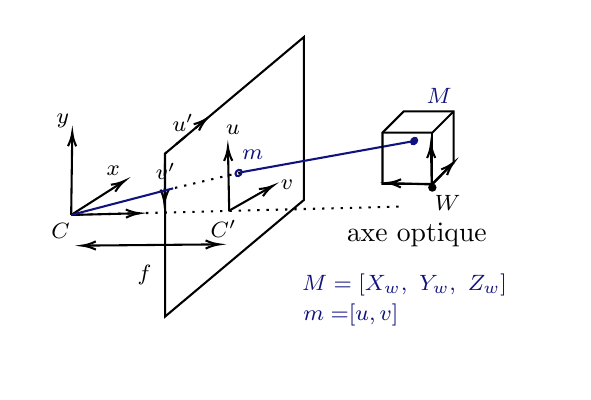
\begin{tikzpicture}[x=0.75pt,y=0.75pt,yscale=-1,xscale=1, scale=0.6]
      
%Shape: Rectangle [id:dp6080383522921334] 
\draw  [line width=0.75]  (261.98,12.03) -- (262.02,142.84) -- (150.52,236.47) -- (150.47,105.66) -- cycle ;
%Shape: Circle [id:dp08023010274775977] 
\draw  [color={rgb, 255:red, 16; green, 18; blue, 125 }  ,draw opacity=1 ][fill={rgb, 255:red, 16; green, 18; blue, 125 }  ,fill opacity=1 ] (350.47,93.07) .. controls (351.83,92.71) and (352.93,93.52) .. (352.93,94.88) .. controls (352.93,96.24) and (351.83,97.64) .. (350.47,98.01) .. controls (349.1,98.37) and (348,97.56) .. (348,96.2) .. controls (348,94.84) and (349.1,93.44) .. (350.47,93.07) -- cycle ;
%Shape: Circle [id:dp3655464346040763] 
\draw  [fill={rgb, 255:red, 0; green, 0; blue, 0 }  ,fill opacity=1 ] (365.12,130.42) .. controls (366.48,130.42) and (367.58,131.52) .. (367.58,132.88) .. controls (367.58,134.25) and (366.48,135.35) .. (365.12,135.35) .. controls (363.75,135.35) and (362.65,134.25) .. (362.65,132.88) .. controls (362.65,131.52) and (363.75,130.42) .. (365.12,130.42) -- cycle ;
%Straight Lines [id:da17745809104725896] 
\draw  [dash pattern={on 4.5pt off 4.5pt}]  (150.02,143.52) -- (150.47,105.66) ;
\draw [shift={(150,145.52)}, rotate = 270.68] [color={rgb, 255:red, 0; green, 0; blue, 0 }  ][line width=0.75]    (10.93,-3.29) .. controls (6.95,-1.4) and (3.31,-0.3) .. (0,0) .. controls (3.31,0.3) and (6.95,1.4) .. (10.93,3.29)   ;
%Straight Lines [id:da05889635157911033] 
\draw  [dash pattern={on 4.5pt off 4.5pt}]  (182.47,78.8) -- (150.47,105.66) ;
\draw [shift={(184,77.52)}, rotate = 139.99] [color={rgb, 255:red, 0; green, 0; blue, 0 }  ][line width=0.75]    (10.93,-3.29) .. controls (6.95,-1.4) and (3.31,-0.3) .. (0,0) .. controls (3.31,0.3) and (6.95,1.4) .. (10.93,3.29)   ;
%Shape: Circle [id:dp5303143417620277] 
\draw  [color={rgb, 255:red, 16; green, 18; blue, 125 }  ,draw opacity=1 ] (209.53,118.71) .. controls (210.9,118.35) and (212,119.15) .. (212,120.52) .. controls (212,121.88) and (210.9,123.28) .. (209.53,123.64) .. controls (208.17,124.01) and (207.07,123.2) .. (207.07,121.84) .. controls (207.07,120.48) and (208.17,119.08) .. (209.53,118.71) -- cycle ;
%Straight Lines [id:da00927428602476521] 
\draw [color={rgb, 255:red, 16; green, 18; blue, 125 }  ,draw opacity=1 ][fill={rgb, 255:red, 16; green, 18; blue, 125 }  ,fill opacity=1 ]   (350.47,95.54) -- (212,120.52) ;
%Straight Lines [id:da32805162479437044] 
\draw    (365.12,130.42) -- (331,129.27) ;
\draw [shift={(329,129.2)}, rotate = 1.93] [color={rgb, 255:red, 0; green, 0; blue, 0 }  ][line width=0.75]    (10.93,-3.29) .. controls (6.95,-1.4) and (3.31,-0.3) .. (0,0) .. controls (3.31,0.3) and (6.95,1.4) .. (10.93,3.29)   ;
%Straight Lines [id:da05612024820893058] 
\draw    (365.12,130.42) -- (380.86,114.19) ;
\draw [shift={(382.25,112.75)}, rotate = 134.12] [color={rgb, 255:red, 0; green, 0; blue, 0 }  ][line width=0.75]    (10.93,-3.29) .. controls (6.95,-1.4) and (3.31,-0.3) .. (0,0) .. controls (3.31,0.3) and (6.95,1.4) .. (10.93,3.29)   ;
%Straight Lines [id:da12713737372353529] 
\draw    (364.65,132.88) -- (364.04,100.2) ;
\draw [shift={(364,98.2)}, rotate = 88.93] [color={rgb, 255:red, 0; green, 0; blue, 0 }  ][line width=0.75]    (10.93,-3.29) .. controls (6.95,-1.4) and (3.31,-0.3) .. (0,0) .. controls (3.31,0.3) and (6.95,1.4) .. (10.93,3.29)   ;
%Shape: Cube [id:dp807415732594561] 
\draw   (325.13,88.8) -- (342.27,71.67) -- (382.25,71.67) -- (382.25,112.75) -- (365.12,129.88) -- (325.13,129.88) -- cycle ; \draw   (382.25,71.67) -- (365.12,88.8) -- (325.13,88.8) ; \draw   (365.12,88.8) -- (365.12,129.88) ;
%Straight Lines [id:da08433615549134643] 
\draw [color={rgb, 255:red, 0; green, 0; blue, 0 }  ,draw opacity=1 ] [dash pattern={on 0.84pt off 2.51pt}]  (338,148.2) -- (75.12,154.88) ;
%Straight Lines [id:da11482119710212657] 
\draw [color={rgb, 255:red, 0; green, 0; blue, 0 }  ,draw opacity=1 ]   (75.12,154.88) -- (75.97,90.75) ;
\draw [shift={(76,88.75)}, rotate = 90.77] [color={rgb, 255:red, 0; green, 0; blue, 0 }  ,draw opacity=1 ][line width=0.75]    (10.93,-3.29) .. controls (6.95,-1.4) and (3.31,-0.3) .. (0,0) .. controls (3.31,0.3) and (6.95,1.4) .. (10.93,3.29)   ;
%Straight Lines [id:da048965394022432385] 
\draw [color={rgb, 255:red, 0; green, 0; blue, 0 }  ,draw opacity=1 ]   (75.12,154.88) -- (116.31,128.59) ;
\draw [shift={(118,127.52)}, rotate = 147.45] [color={rgb, 255:red, 0; green, 0; blue, 0 }  ,draw opacity=1 ][line width=0.75]    (10.93,-3.29) .. controls (6.95,-1.4) and (3.31,-0.3) .. (0,0) .. controls (3.31,0.3) and (6.95,1.4) .. (10.93,3.29)   ;
%Straight Lines [id:da0181640786884405] 
\draw [color={rgb, 255:red, 0; green, 0; blue, 0 }  ,draw opacity=1 ]   (75.12,154.88) -- (128,153.57) ;
\draw [shift={(130,153.52)}, rotate = 178.57] [color={rgb, 255:red, 0; green, 0; blue, 0 }  ,draw opacity=1 ][line width=0.75]    (10.93,-3.29) .. controls (6.95,-1.4) and (3.31,-0.3) .. (0,0) .. controls (3.31,0.3) and (6.95,1.4) .. (10.93,3.29)   ;
%Straight Lines [id:da4676436047615513] 
\draw [color={rgb, 255:red, 16; green, 18; blue, 125 }  ,draw opacity=1 ]   (157,133.52) -- (75.12,154.88) ;
%Straight Lines [id:da7951596067163212] 
\draw [color={rgb, 255:red, 0; green, 0; blue, 0 }  ,draw opacity=1 ]   (86,179.5) -- (192,178.53) ;
\draw [shift={(194,178.52)}, rotate = 179.48] [color={rgb, 255:red, 0; green, 0; blue, 0 }  ,draw opacity=1 ][line width=0.75]    (10.93,-3.29) .. controls (6.95,-1.4) and (3.31,-0.3) .. (0,0) .. controls (3.31,0.3) and (6.95,1.4) .. (10.93,3.29)   ;
\draw [shift={(84,179.52)}, rotate = 359.48] [color={rgb, 255:red, 0; green, 0; blue, 0 }  ,draw opacity=1 ][line width=0.75]    (10.93,-3.29) .. controls (6.95,-1.4) and (3.31,-0.3) .. (0,0) .. controls (3.31,0.3) and (6.95,1.4) .. (10.93,3.29)   ;
%Straight Lines [id:da4782896820641106] 
\draw [color={rgb, 255:red, 0; green, 0; blue, 0 }  ,draw opacity=1 ] [dash pattern={on 0.84pt off 2.51pt}]  (211.07,120.84) -- (157,133.52) ;
%Shape: Rectangle [id:dp446540245188062] 
\draw  [color={rgb, 255:red, 255; green, 255; blue, 255 }  ,draw opacity=1 ] (41.02,5.34) -- (469,5.34) -- (469,280.34) -- (41.02,280.34) -- cycle ;
%Straight Lines [id:da18381069731153055] 
\draw    (202.02,152.01) -- (201.04,102.52) ;
\draw [shift={(201,100.52)}, rotate = 88.86] [color={rgb, 255:red, 0; green, 0; blue, 0 }  ][line width=0.75]    (10.93,-3.29) .. controls (6.95,-1.4) and (3.31,-0.3) .. (0,0) .. controls (3.31,0.3) and (6.95,1.4) .. (10.93,3.29)   ;
%Straight Lines [id:da04744764226882381] 
\draw    (202.56,151.13) -- (235.26,132.51) ;
\draw [shift={(237,131.52)}, rotate = 150.34] [color={rgb, 255:red, 0; green, 0; blue, 0 }  ][line width=0.75]    (10.93,-3.29) .. controls (6.95,-1.4) and (3.31,-0.3) .. (0,0) .. controls (3.31,0.3) and (6.95,1.4) .. (10.93,3.29)   ;

% Text Node
\draw (358,50.9) node [anchor=north west][inner sep=0.75pt]  [font=\footnotesize,color={rgb, 255:red, 16; green, 18; blue, 125 }  ,opacity=1 ]  {$M$};
% Text Node
\draw (364.65,136.28) node [anchor=north west][inner sep=0.75pt]  [font=\footnotesize]  {$W$};
% Text Node
\draw (154,71.9) node [anchor=north west][inner sep=0.75pt]  [font=\footnotesize]  {$u'$};
% Text Node
\draw (129.5,109.4) node [anchor=north west][inner sep=0.75pt]  [font=\footnotesize]  {$ \begin{array}{l}
v'\\
\end{array}$};
% Text Node
\draw (210,99.9) node [anchor=north west][inner sep=0.75pt]  [font=\footnotesize,color={rgb, 255:red, 167; green, 17; blue, 17 }  ,opacity=1 ]  {$\textcolor[rgb]{0.06,0.07,0.49}{m}$};
% Text Node
\draw (294,159) node [anchor=north west][inner sep=0.75pt]   [align=left] {axe optique};
% Text Node
\draw (126,192.9) node [anchor=north west][inner sep=0.75pt]  [font=\footnotesize]  {$f$};
% Text Node
\draw (56.65,159.28) node [anchor=north west][inner sep=0.75pt]  [font=\footnotesize]  {$C$};
% Text Node
\draw (61,70.9) node [anchor=north west][inner sep=0.75pt]  [font=\footnotesize]  {$y$};
% Text Node
\draw (101,112.9) node [anchor=north west][inner sep=0.75pt]  [font=\footnotesize]  {$x$};
% Text Node
\draw (184.65,156.6) node [anchor=north west][inner sep=0.75pt]  [font=\footnotesize]  {$C'$};
% Text Node
\draw (241,123.9) node [anchor=north west][inner sep=0.75pt]  [font=\footnotesize]  {$v$};
% Text Node
\draw (197,79.92) node [anchor=north west][inner sep=0.75pt]  [font=\footnotesize]  {$u$};
% Text Node
\draw (258,199.9) node [anchor=north west][inner sep=0.75pt]  [font=\footnotesize,color={rgb, 255:red, 16; green, 18; blue, 125 }  ,opacity=1 ]  {$M=[ X_{w} ,\ Y_{w} ,\ Z_{w}]$};
% Text Node
\draw (259,223.9) node [anchor=north west][inner sep=0.75pt]  [font=\footnotesize,color={rgb, 255:red, 167; green, 17; blue, 17 }  ,opacity=1 ]  {$\textcolor[rgb]{0.06,0.07,0.49}{m=}\textcolor[rgb]{0.06,0.07,0.49}{[}\textcolor[rgb]{0.06,0.07,0.49}{u,v}\textcolor[rgb]{0.06,0.07,0.49}{]}$};


    \end{tikzpicture}
  \end{overlayarea}
\end{minipage}
\end{frame}


\begin{frame}[noframenumbering]{Projection d’un point 3D sur le plan image}
  \centering
  \[
    \begin{bmatrix}
    u \\ v \\ w
    \end{bmatrix}
    =
    \underbrace{
    \begin{bmatrix}
    f & 0 & 0 & 0 \\
    0 & f & 0 & 0 \\
    0 & 0 & 1 & 0
    \end{bmatrix}
    \begin{bmatrix}
    R & T \\
    0 & 1
    \end{bmatrix}
    }_{\text{chaîne de projection}}
    \begin{bmatrix}
    X_w \\ Y_w \\ Z_w \\ 1
    \end{bmatrix}
  \]
  
  \pause
  \[
    \begin{bmatrix}
    u \\ v \\ w
    \end{bmatrix}
    =
    P
    \begin{bmatrix}
    X_w \\ Y_w \\ Z_w \\ 1
    \end{bmatrix}
    \quad \text{avec} \quad
    P \in \mathcal{M}_{3 \times 4}(\mathbb{R})
  \]
\end{frame}



%-----------------------------------------------
\begin{frame}[noframenumbering]{Les différents repères}

\[
\lambda_i 
\begin{pmatrix}
u^{(i)} \\
v^{(i)} \\
1
\end{pmatrix}
=
\begin{pmatrix}
p_{11} & p_{12} & p_{13} & p_{14} \\
p_{21} & p_{22} & p_{23} & p_{24} \\
p_{31} & p_{32} & p_{33} & p_{34}
\end{pmatrix}
\begin{pmatrix}
x_C^{(i)} \\
y_C^{(i)} \\
z_C^{(i)} \\
1
\end{pmatrix}
\]
\end{frame}

\begin{frame}[noframenumbering]{Système d’optimisation à contrainte unitaire}
\label{optimisation-appendix}
On souhaite résoudre le système en évitant la solution triviale \( P = 0 \).  
\pause

Sachant que la matrice \( P \) ne peut être déterminée qu’à un facteur près, on peut imposer :
\[
\|P\|^2 = 1
\]
et reformuler le système comme un problème d’optimisation :
\pause
\[
\min_{\|p\|^2 = 1} \|Ap\|^2 = \min_{\|p\|^2 = 1} p^T A^T A p
\]
\pause
On introduit les fonctions :
\begin{itemize}
  \item \( f(p) = p^T A^T A p \)
  \item \( g(p) = p^T p - 1 \)
\end{itemize}
\pause
D’après le théorème d’optimisation sous contrainte (Lagrange), au point optimal \( P^* \), il existe \( \lambda \in \mathbb{R} \) tel que :
\[
\nabla f(P^*) = \lambda \nabla g(P^*)
\]
\end{frame}



\begin{frame}[noframenumbering]{Lien avec les valeurs propres}

Posons \( M = A^T A \).  
Alors :
\[
f(p) = \sum_{i=1}^n \sum_{j=1}^n p_i M_{ij} p_j
\]
\pause

Comme \( M \) est symétrique :
\[
\frac{\partial f}{\partial p} = 2Mp
\quad \text{et} \quad
\frac{\partial g}{\partial p} = 2p
\]
\pause

On a donc :
\[
\frac{\partial f}{\partial p} = \lambda \frac{\partial g}{\partial p}
\quad \Rightarrow \quad
\boxed{A^T A p = \lambda p}
\]
\pause

C’est une équation aux valeurs propres :
\begin{itemize}
  \item \( p \) est un vecteur propre de \( A^T A \)
  \item \( \lambda \) est la valeur propre associée
\end{itemize}
\end{frame}

\begin{frame}[noframenumbering]{Triangulation : formulation du système}
\vspace*{-0.5em}
\begin{itemize}
  \item<1-> \( P_1 \) et \( P_2 \) déterminées
  \item<2-> On cherche les coordonnées \( X = (x_C, y_C, z_C, 1)^T \)
  \item<3-> Pour chaque paire \( (x_1, x_2) \) de projections
  \item<4-> On élimine \( \lambda_1, \lambda_2 \) et on écrit un système homogène
  \item<5-> Système sous la forme \( A X = 0 \)
\end{itemize}

\vspace{1em}

\pause
\pause
\pause
\pause
\begin{center}
\scriptsize
\[
A =
\left(
\begin{array}{cccc}
p_{31}^{1} u_1 - p_{11}^{1} & p_{32}^{1} u_1 - p_{12}^{1} & p_{33}^{1} u_1 - p_{13}^{1} & p_{34}^{1} u_1 - p_{14}^{1} \\
p_{31}^{1} v_1 - p_{21}^{1} & p_{32}^{1} v_1 - p_{22}^{1} & p_{33}^{1} v_1 - p_{23}^{1} & p_{34}^{1} v_1 - p_{24}^{1} \\
p_{31}^{2} u_2 - p_{11}^{2} & p_{32}^{2} u_2 - p_{12}^{2} & p_{33}^{2} u_2 - p_{13}^{2} & p_{34}^{2} u_2 - p_{14}^{2} \\
p_{31}^{2} v_2 - p_{21}^{2} & p_{32}^{2} v_2 - p_{22}^{2} & p_{33}^{2} v_2 - p_{23}^{2} & p_{34}^{2} v_2 - p_{24}^{2}
\end{array}
\right)
\]
\vspace*{1cm}
\end{center}
\end{frame}



\begin{frame}[noframenumbering]
    \scriptsize
    \begin{algorithm}[H]
\DontPrintSemicolon
\Input{$A \in \mathbb{R}^{m \times n}$}
\Output{$Q \in \mathbb{R}^{m \times n}$, $R \in \mathbb{R}^{n \times n}$ tels que $A = QR$}
\BlankLine

\For{$j \gets 1$ \KwTo $n$}{
  $v_j \gets A_{:,j}$ \tcc*[r]{Copie de la $j^{\text{\`e}me}$ colonne de $A$}
  \For{$i \gets 1$ \KwTo $j-1$}{
    $R_{i,j} \gets \langle Q_{:,i}, A_{:,j} \rangle$ \;
    $v_j \gets v_j - R_{i,j} Q_{:,i}$ \;
  }
  $R_{j,j} \gets \|v_j\|$ \;
  \Si{$R_{j,j} > \varepsilon$}{
    $Q_{:,j} \gets \frac{v_j}{R_{j,j}}$
  }
  \Sinon{
    $Q_{:,j} \gets 0$
  }
}
\Return{$Q, R$}
\caption{Décomposition QR via Gram-Schmidt}
\end{algorithm}
\end{frame}

%------------------------

\begin{frame}[noframenumbering]
  \label{SVD-appendix}
\scriptsize
\begin{algorithm}[H]
\DontPrintSemicolon
\Input{$B \in \mathbb{R}^{n \times n}$ symétrique}
\Output{$\Sigma^2$, $V$ tels que $B = V \Sigma^2 V^T$}

\BlankLine
$Q_{\text{acc}} \gets I_n$ \tcc*[r]{Accumule les produits de $Q$}
\BlankLine
%$\varepsilon \gets 10^{-12}$ \;
$\delta \gets 1$, $k_{\text{max}} \gets 1000$, $k \gets 0$\;

\Tq{$\delta > 10^{-9}$ et $k < k_{\text{max}}$}{
  $Q, R \gets$ décomposition QR de $B$\;
  $B_{\text{nouveau}} \gets R \cdot Q$\;
  $Q_{\text{acc}} \gets Q_{\text{acc}} \cdot Q$\;

  $\delta \gets \sum_i |\text{diag}(B_{\text{nouveau}})_i - \text{diag}(B)_i|$\;

  $A \gets B_{\text{nouveau}}$\;
  $k \gets k + 1$\;
}

\BlankLine
\For{$i=1$ à $n$}{
  \Si{$1[i, i] > \varepsilon$}{
    $\Sigma^2[i, i] \gets V[i, i]$
  }
  \Sinon{
    $\Sigma^2[i, i] \gets 0$
  }
}

\Return{$\Sigma^2$,$Q_{\text{acc}}$ }

\caption{algorithme QR}
\end{algorithm}
\end{frame}

\begin{frame}[noframenumbering]
\scriptsize  
\begin{algorithm}[H]
\DontPrintSemicolon
\Input{$A \in \mathbb{R}^{m \times n}$}
\Output{$U, \Sigma, V$ tels que $A \approx U \Sigma V^T$}

\BlankLine
$A^T \gets$ transposée de $A$\;
$A^T A \gets A^T \cdot A$ \tcc*[r]{Symétrique et définie positive}

\BlankLine
\texttt{algorithme\_QR}($A^T A$, $\Sigma^2$, $V$) \tcc*[r]{$\Sigma^2$ diagonale, $V$ orthogonale}

\BlankLine
\For{$i \gets 1$ \KwTo $n$}{
    $\sigma^2 \gets \Sigma^2[i, i]$\;
    \Si{$\sigma^2 < 10^{-12}$}{
        \textbf{continuer} \tcc*[r]{Ignorer valeur singulière nulle}
    }

    $\sigma \gets \sqrt{\sigma^2}$\;
    $\Sigma[i, i] \gets \sigma$ \tcc*[r]{Met à jour la vraie valeur singulière}

    $v_i \gets$ $i^{\text{e}}$ colonne de $V$\;
    $u_i \gets A \cdot v_i$ \tcc*[r]{$u_i$ non normalisé}
    $u_i \gets u_i / \sigma$\;
    normaliser $u_i$\;
    insérer $u_i$ comme $i^{\text{e}}$ colonne de $U$\;
}

\caption{SVD via algorithme QR sur \( A^T A \)}
\end{algorithm}
\end{frame}

\begin{frame}[noframenumbering]{Ransac}
  \label{ransac-appendix}
    \begin{columns}
        \begin{column}{0.5\textwidth}
            \centering
            \begin{tikzpicture}[scale=1]

                % --- Tous les points initiaux ---
                \only<1-3>{
                    \foreach \x/\y in {
                        0.5/1.0, 1.0/1.2, 1.5/1.3, 2.0/1.7, 2.5/2.1, 3.0/2.1, 3.5/2.4, 4.0/2.8,
                        1.0/3.5, 2.0/3.7, 3.0/3.9, 4.0/4.2
                    } {
                        \filldraw[blue!70!black] (\x,\y) circle (2pt);
                    }
                }

                % --- Points restants (extrémités et bruit) ---
                \only<4->{
                    \foreach \x/\y in {
                        1.0/3.5, 2.0/3.7, 3.0/3.9, 4.0/4.2
                    } {
                        \filldraw[blue!70!black] (\x,\y) circle (2pt);
                    }
                }

                % Droite testée
                \only<3->{
                    \draw[thick, red, dashed] (0.3,0.8) -- (4.5,3.0);
                }

                % Points choisis
                \only<2-3>{
                    \filldraw[red] (1.5,1.3) circle (3pt);
                    \filldraw[red] (3.0,2.1) circle (3pt);
                }

                % Inliers détectés
                \only<3>{
                    \foreach \x/\y in {
                        0.5/1.0, 1.0/1.2, 2.0/1.7, 2.5/2.1, 3.5/2.4, 4.0/2.8
                    } {
                        \filldraw[green!50!black] (\x,\y) circle (2.5pt);
                    }
                }

                % Points supprimés
                \only<4>{
                    \foreach \x/\y in {
                        1.0/1.2, 2.0/1.7, 2.5/2.1, 3.5/2.4
                    } {
                        \node[draw=red, cross out, thick, minimum size=6pt, inner sep=0pt] at (\x,\y) {};
                    }
                }

                % Points extrémités conservés (surlignés)
                \only<4->{
                    \filldraw[black] (0.5,1.0) circle (3pt);
                    \filldraw[black] (4.0,2.8) circle (3pt);
                }

            \end{tikzpicture}
        \end{column}

        \begin{column}{0.5\textwidth}
            \small
            \begin{itemize}
                \item<1-> Points d’entrée dans le nuage
                \item<2-> Sélection de deux points pour estimer une droite
                \item<3-> Inliers détectés à proximité de la droite
                \item<4-> Suppression des points internes, on garde les extrémités
            \end{itemize}

            \vspace{0.5em}
            \only<4>{
                \textcolor{red}{\small $\Rightarrow$ Nettoyage effectué : seuls les segments visibles sont conservés}
            }
        \end{column}
    \end{columns}
\end{frame}


\begin{frame}{Points d'intérêts}
  \label{convex-appendix}
\note{
Pour un objet convexe tel qu'un cube, il nous suffit de répérer ces sommets pour le reconstruir en 3D.
Mais si l’objet est non convexe, comme dans le schéma de droite, on peut détecter des coins qui ne sont pas représentatifs de la structure globale.
On voit ici que l’enveloppe convexe (en bleu) ne correspond pas exactement à la forme réelle. Ce genre de situation peut gêner certaines étapes de reconstruction.
On s'est ainsi fixé une contrainte de convexité qui nous permet de définir les points d'intérets comme les points correspondants aux sommet de l'objet su'on souhaite reconstruire
}
\begin{minipage}[t]{0.48\textwidth}
\centering
\textbf{Points d'intérêts  sur un cube}\\[0.5em]
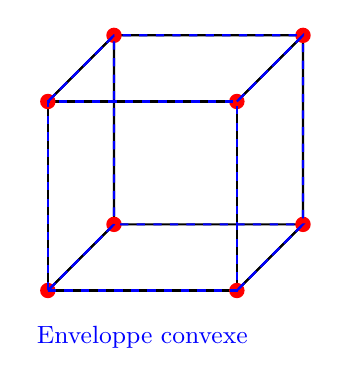
\begin{tikzpicture}[scale=1.2]

% Cube en perspective
\coordinate (A) at (0,0);
\coordinate (B) at (2,0);
\coordinate (C) at (2,2);
\coordinate (D) at (0,2);
\coordinate (E) at (0.7,0.7);
\coordinate (F) at (2.7,0.7);
\coordinate (G) at (2.7,2.7);
\coordinate (H) at (0.7,2.7);

% Faces du cube
\draw[thick] (A) -- (B) -- (C) -- (D) -- cycle; % face avant
\draw[thick] (A) -- (E) -- (F) -- (B); % face basse
\draw[thick] (B) -- (F) -- (G) -- (C);
\draw[thick] (C) -- (G) -- (H) -- (D);
\draw[thick] (D) -- (H) -- (E) -- (A);

\pause
% Coins détectés
\foreach \pt in {(A), (B), (C), (D), (E), (F), (G), (H)} {
  \filldraw[red] \pt circle (2pt);
}

\pause
% Enveloppe convexe

\draw[blue, dashed, thick]  (A) -- (B) -- (C) -- (D) -- cycle; % face avant
\draw[blue, dashed, thick]  (A) -- (E) -- (F) -- (B); % face basse
\draw[blue, dashed, thick]  (B) -- (F) -- (G) -- (C);
\draw[blue, dashed, thick]  (C) -- (G) -- (H) -- (D);
\draw[blue, dashed, thick]  (D) -- (H) -- (E) -- (A);

\node[blue] at (1,-0.5) {\small Enveloppe convexe};

\end{tikzpicture}
\end{minipage}
\hfill
\begin{minipage}[t]{0.48\textwidth}
\centering
\only<3->{
\pause
\textbf{Problème si non convexe}\\[0.5em]
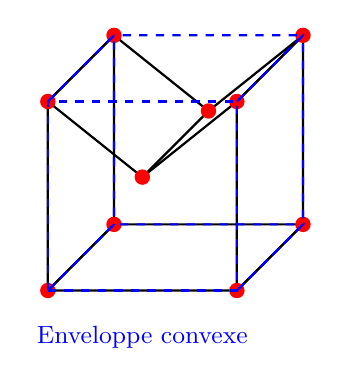
\begin{tikzpicture}[scale=1.2]
% Cube en perspective
\coordinate (A) at (0,0);
\coordinate (B) at (2,0);
\coordinate (B2) at (1,1.2);
\coordinate (C2) at (1.7,1.9);
\coordinate (C) at (2,2);
\coordinate (D) at (0,2);
\coordinate (E) at (0.7,0.7);
\coordinate (F) at (2.7,0.7);
\coordinate (G) at (2.7,2.7);
\coordinate (H) at (0.7,2.7);

% Faces du cube
\draw[thick] (A) -- (B) -- (C) -- (B2) -- (D) -- cycle; % face avant
\draw[thick] (A) -- (E) -- (F) -- (B); % face basse
\draw[thick] (B) -- (F) -- (G) -- (C);
\draw[thick] (C) -- (G) -- (C2)-- (H) -- (D);
\draw[thick] (D) -- (H) -- (E) -- (A);
\draw[thick] (B2) -- (C2);

\pause
% Coins détectés
% Coins détectés
\foreach \pt in {(A), (B), (C), (D), (E), (F), (G), (H), (B2),(C2)} {
  \filldraw[red] \pt circle (2pt);
}


\pause
% Enveloppe convexe

\draw[blue, dashed, thick]  (A) -- (B) -- (C) -- (D) -- cycle; % face avant
\draw[blue, dashed, thick]  (A) -- (E) -- (F) -- (B); % face basse
\draw[blue, dashed, thick]  (B) -- (F) -- (G) -- (C);
\draw[blue, dashed, thick]  (C) -- (G) -- (H) -- (D);
\draw[blue, dashed, thick]  (D) -- (H) -- (E) -- (A);

\node[blue] at (1,-0.5) {\small Enveloppe convexe};
\end{tikzpicture}
}
\end{minipage}
\end{frame}


\begin{frame}{Resultat : Filtrage epipolaire}
  \label{brief-appendix}
  \hspace*{-1cm}
  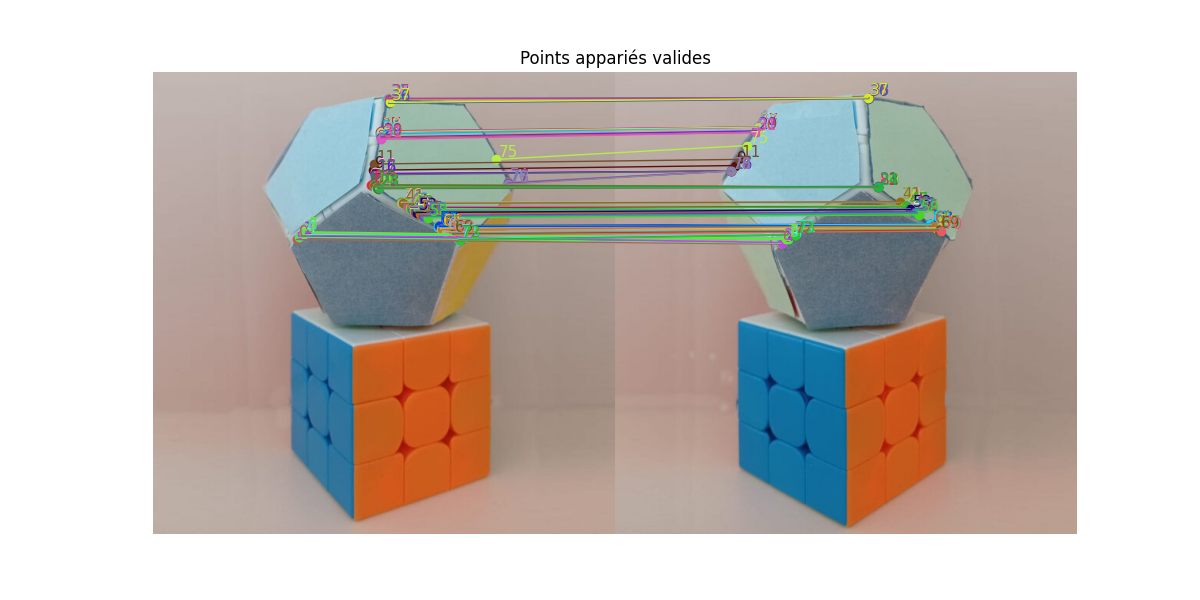
\includegraphics[width=1.1\linewidth]{capture/sans_brief.png}\\[0.5em]
\end{frame}

\begin{frame}{Resultat : droite epipolaire + BRIEF lab}
  \hspace*{-1cm}
  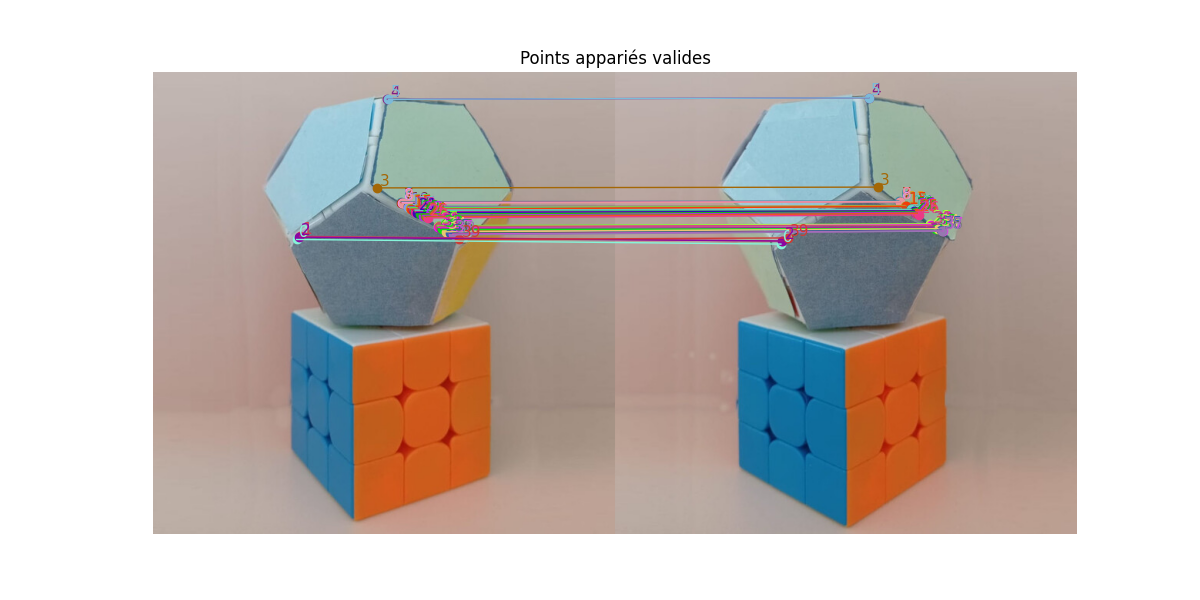
\includegraphics[width=1.1\linewidth]{capture/avec_brief.png}\\[0.5em]
\end{frame}

% \begin{frame}{Paramètres}
% \label{param-appendix}
% \ttfamily
% \textbf{Appariement}
% int Distance_seuil = 4;
% int Hamming_seuil = 45;
% \textbf{Détection}
% int Window = 4;
% int Seuil_moravec = 800;
% \textbf{RANSAC}
% int RANSAC_ITER = 1000;
% int DIST_THRESHOLD = 1.0;
% int MIN_INLIERS = 5;
% \textbf{Trouve coin}
% int Seuil_tc = 40;
% int Dist_tc = 10
% \end{frame}